%%%%%%%%%%%%%%%%%%%%%%%%%%%%%%%%%%%%%%%%%%%%%%%%%%%%%%%%%%%
% EPFL report package, main thesis file
% Goal: provide formatting for theses and project reports
% Author: Mathias Payer <mathias.payer@epfl.ch>
%
% To avoid any implication, this template is released into the
% public domain / CC0, whatever is most convenient for the author
% using this template.
%
%%%%%%%%%%%%%%%%%%%%%%%%%%%%%%%%%%%%%%%%%%%%%%%%%%%%%%%%%%%
\documentclass[a4paper,11pt,oneside]{report}
% Options: MScThesis, BScThesis, MScProject, BScProject
\usepackage[MScProject]{EPFLreport}
\usepackage{xspace}

\title{Design and evaluation of mixers\\in a high-churn environment}
\author{Derya Cögendez}
\supervisor{Linus Gasser}
\adviser{Pierluca Borsò-Tan}
%\coadviser{Second Adviser}
\newcommand{\sysname}{FooSystem\xspace}

\begin{document}
\maketitle
\makeacks

\begin{abstract}
Fledger is a peer-to-peer network that runs on browsers, it is very modular an can easily be extended with additional services. One of it's services, web proxy, enables peers to act as proxies for other nodes. This service can provide some additional privacy for the users, and depending on the rules enforced by the proxy, additional security. However it does not to protect from traffic analysis by an adversary observing the network nor does it hide traffic patterns from the proxy node. In this project, review existing anonymous communication systems that can be used for this specific case of a web proxy. We create a proof of concept implementation and fine tune and evaluate it in the setting of Fledger. In addition, we try to improve the reliability of the web proxy requests with this implementation in the inevitable presence of churn by the use of simple mechanism such as retrying and sending duplicate messages.
\textbf{Add a few sentences about the results here}
\end{abstract}

\maketoc

%%%%%%%%%%%%%%%%%%%%%%
\chapter{Introduction}
%%%%%%%%%%%%%%%%%%%%%%
% The introduction is a longer writeup that gently eases the reader into your
% thesis~\cite{dinesh20oakland}. Use the first paragraph to discuss the setting.
% In the second paragraph you can introduce the main challenge that you see.
% The third paragraph lists why related work is insufficient.
% The fourth and fifth paragraphs discuss your approach and why it is needed.
% The sixth paragraph will introduce your thesis statement. Think how you can
% distill the essence of your thesis into a single sentence.
% The seventh paragraph will highlight some of your results
% The eights paragraph discusses your core contribution.

% This section is usually 3-5 pages.
\textbf{Insert something that leads onto fledger or something about web proxies}

Fledger\textbf{cite} is a peer-to-peer network designed to work directly in the browser, without the need for proxies. It enables connecting browsers to communicate between nodes. It is under development and will let users share resources like disk space, CPU, and network bandwidth in the future. Fledger's initial use cases are a decentralized chat application and web proxy. Although with the current version of Fledger, one can use the web proxy, there are some privacy concerns with it. Although using a web proxy can reveal less information about internet use of the user to their ISP, this time the proxy node can learn about the traffic patterns of the user. Since the proxy request does not hide the address of the user and multiple proxy requests from the same node will reveal information about the web traffic pattern of the user. The web proxy service also doesn't provide any privacy protections against an observer of the peer-to-peer network.

\textbf{Talk about what the project was about}
% To remedy this issue, this project looks into different anonymous communications systems. 

% The first anonymous communication system that comes to mind, Tor\textbf{cite}, is vulrable to traffic analysis [cite stuff].
% % To our knowledge there isn't much research into using mixnets for web surfing as for a long time mixnetwork have been limited by their high latency.
% % Can probably get some inpiration from one of the mixnet papers
% Other communications systems such as .... although solves the problem of Tor, they usually have very high latencies unsuitable for an "instantanous" application such as a web proxy.

% We choose Loopix Anonymity System \textbf{cite} for it's low latency, apparent scalability (and tunability) and availability of reference implementations.

% We integrate Loopix into Fledger, and adapt it for use for the specific purpose of web browsing through a web proxy. We then choose configuration parameters through extensive experimentation. Although the Loopix paper looks extensively into the privacy aspects of the system, they leave reliable message delivery to future work. \textbf{transition} We explore potential ways to improve the reliability of our implementation. Finally we add simple mechanisms to have more reliable message delivery in the presence of churn.

% In conclusion:

% Conclusion: integrated loopix anonymity system into fledger and adapted it for the specific purpose of web proxying with low latency and high reliability. 

%%%%%%%%%%%%%%%%%%%%
\chapter{Background}
%%%%%%%%%%%%%%%%%%%%

% The background section introduces the necessary background to understand your
% work. This is not necessarily related work but technologies and dependencies
% that must be resolved to understand your design and implementation.

% This section is usually 3-5 pages.

%-------------------
\section{Fledger}
%-------------------
Fledger is a P2P network that can be run entirely using browsers, it's goal is to enable user to share resources such as CPU, bandwidth, disk space etc. It runs the WebRTC protocol to communicate and uses a Signaling Server to enable nodes to discover each other and establish connections. Although it can be run entrirely using browsers, Fledger nodes can also be run as standalone nodes. This project is a fork of Fledger \textbf{cite github repository}
%-------------------
\subsection{Communication between nodes}

When a new Fledger node joins the network, it creates a key pair and derives and ID from it. This ID is called a nodeID, it is nodeID is the main routing information for Fledger nodes. 

After the node starts up and creates its routing information, it announces itself to the Signaling server, which in turn gives the node information about other nodes that are online.

When the node wants to communicate with another node, it will send a message to the signaling server. The signaling server will act as a mediator for the two nodes to negotiate a connection. Once the connection is established between the nodes, they can communicate through their browsers.

In \autoref{fig:webrtc}, Peer 1 sends a message to the Signaling server to start establishing a connection with Peer 2, they communicate through the signaling server to negotiate the connection. Once the connection is established, they can directly communicate without the need for the Signaling server. 

\begin{figure}[H]
    \centering
    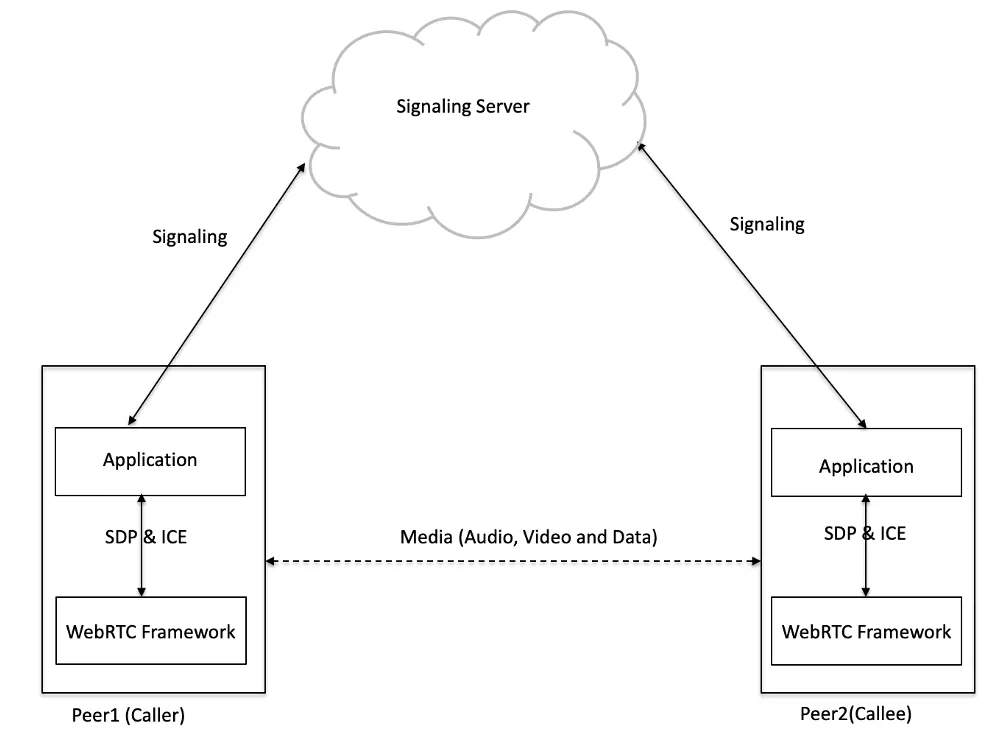
\includegraphics[width=0.8\linewidth]{plots/webrtc.png}
    \caption{}
    \label{fig:webrtc}
    \small\textit{Figure from Medium: "Choice of Signaling Server in Web Real-Time Communication"}
\end{figure}

%-------------------
\subsection{Modules}
\label{sec:fledger_modules}

For each functionality in Fledger, there is a separate module. This section will introduce the relevant Fledger modules to this project.

\begin{itemize}
    \item \textbf{Network}\\
    Network module uses the WebRTC protocol and enables other modules send messages through its messages. It can be used for both browsers and for Fledger nodes. In this project we use Fledger as 
    \item \textbf{Gossip and Random Connections Modules} \\
    Gossiping module enables messages to be propagated through the Fledger network, and it uses Random Connections module. Random Connections module is designed to establish random connections between the nodes, and it uses the network module to send messages to the selected nodes. These two module are used for the bootstrapping of the Loopix Module for the purpose of experimentation. See \autoref{sec:design_bootstrapping} for further details about the bootstrapping.
    \item \textbf{Web Proxy}\\
    Web proxy module handles web proxy requests, it can be used to create and respond to request to get web pages. It creates a unique ID for a request and sends the message. When a node responds to a request, it sends multiple messages with the same unique ID as the request, which enables the web proxy client to collect the messages into the requested page. If the client does not receive the complete response within a set period of time, the request will timeout.
    \item \textbf{Overlay}\\
    This module acts as a translator/wrapper for Fledger modules. While sending a message through gossip or web proxy this module will wrap the message and then send it to the specific module. For example if node A wants to send a web proxy message to node B, node A will create web proxy message, which will be sent to Overlay module, still within node A, and Overlay module will translate for the corresponding module, for example random connections, and send the translated message to this module, which will finally send the message to the network module, and the message will be sent to node B through the WebRTC connection. Linus Gasser has kindly created this module to help integrate Loopix module into Fledger.
    \item \textbf{Loopix}\\
    In this project we have created a Loopix module that can be used as a middle man between any module and the network module. The main purpose is to be used with web proxy but it can be used to send other kinds of messages from Fledger modules as long as they are sent through an Overlay.
\end{itemize}

%-------------------
\section{The Loopix Anonymity System}
\label{sec:loopix}
%-------------------
This section will give a summary of the Loopix Anonymity System introduced in \textbf{cite}. Loopix is a continuous time mix network. Unlike the traditional mix networks introduced by \textbf{cite chaum}, in continuous time mix networks, which operate in rounds. Packets are stopped for a specified delay at the mix node and then sent on their ways. This delay is usually drawn from an exponential dsitribution \textbf{cite}.

Loopix combines this stop-and-go mixing with cover traffic to further hide traffic patterns and avoid flooding attacks (n-1)\textbf{cite}, which were possible with round based mix networks.

Quite like the Tor network, the route of the message is chosen by the user in advance and the messages are encapsulated in layers of encryption with public keys each of node in the route. However, unlike the Tor network, each message goes through a separate route, with a different delay at each node in the route. These delays combined with separate routes, make it harder to perform traffic analysis by observing entry and exit nodes, which is quite trivial with Tor \textbf{cite}.

The Loopix network consists of three different roles. Nodes that use the mix network are referred to as clients. Each client chooses a provider, which serves as the entry point to the network for that client. A client routes all of its traffic through its provider, which, in turn, forwards the client’s messages to the mix network. Additionally, the provider stores any messages destined for its client. When the client is online, it retrieves these stored messages from its provider.

Finally, there are mix nodes. Mix nodes are arranged in a stratified topology \textbf{cite}, and their main purpose is to remove a layer of encryption from the messages that they receive, wait for a delay which is specified in the header of the decrypted packet, and then send the message to the next node in its route. The mix node only knows about the delay, and previous and next nodes.

\begin{figure}[H]
    \centering
    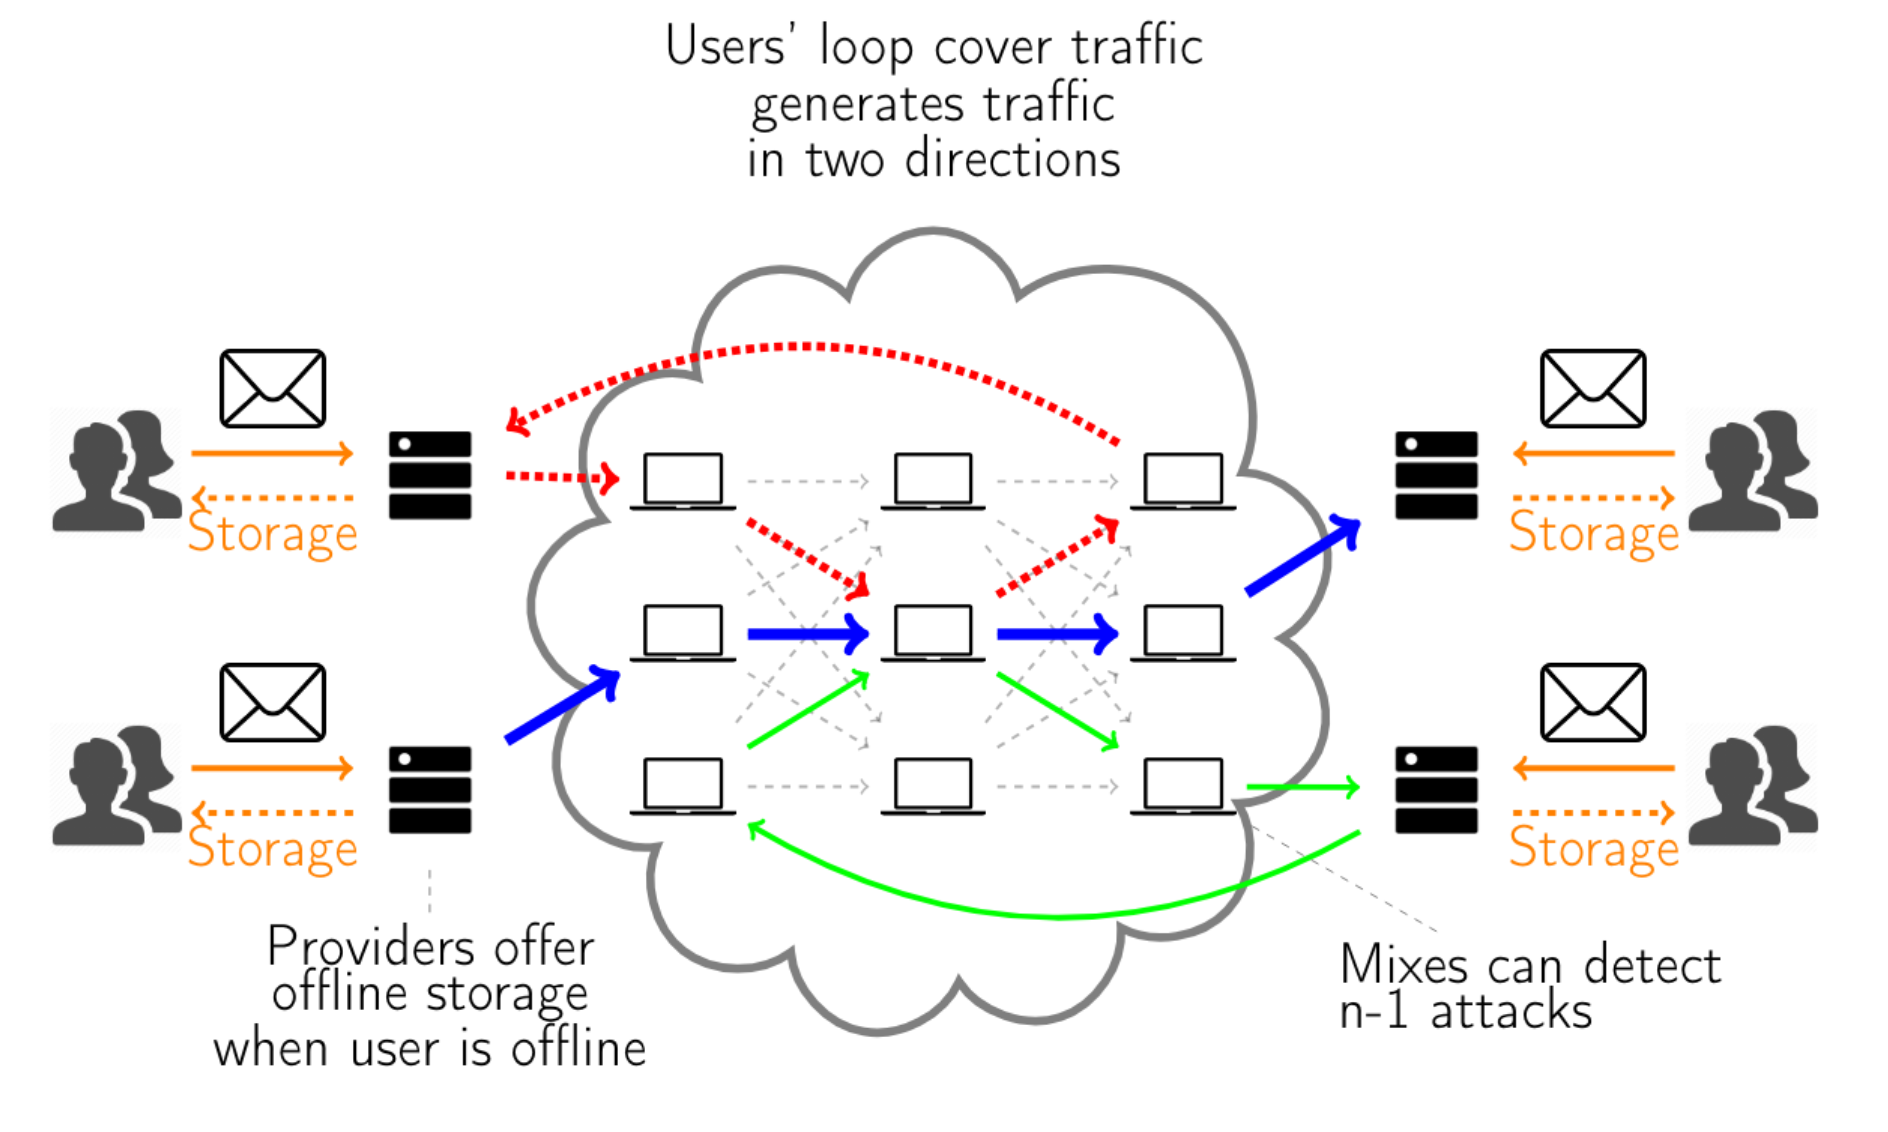
\includegraphics[width=0.8\linewidth]{plots/loopix.png}
    \caption{}
    \label{fig:loopix}
    \small\textit{Figure 1 from The Loopix Anonymity System paper}
\end{figure}

\textbf{TODO get rid of the text at the top of the figure}

The typical route of a message from a client goes to their provider, who forwards it to the mix node at the first layer of the stratified topology. Each mix node at each layer of the mix network, receives and forwards this message, until it arrives at the provider of the destination client. The destination provider stores the message, until the client retrieves it. Of course, creating this route requires the source client to know the addresses of mix nodes at each layer as well as the destination client and the provider of the destination.

\textbf{TODO mention sphinx packets}
%-------------------
\subsection{Types of Messages}
\begin{itemize}
    \item \textbf{Subscribe Message} \\
    When a client joins the network client sends a subscribe message to a provider of its own choosing. When a provider receives a subscribe message, it simply adds the client to its list of subscribed clients and stores any messages that arrive for this client.
    \item \textbf{Payload Message} \\
    If a client want to send a real message to another client, it creates a payload message. These payload messages are then put into a queue and the client pops messages from this queue at a constant rate.
    \item \textbf{Drop Message} \\
    If the client payload message queue is empty, the client sends a drop message instead. These message are sent to a random random provider and they are dropped at the destination. All nodes, clients, providers, and mix nodes, periodically send drop messages.
    \item \textbf{Loop Message} \\
    Loop messages give the Loopix anonymity system its name. They are part of the cover traffic along with the drop messages. Loop messages are sent by a node to itself, routed through a random provider. They simulate receiving a reply to a message, and provide important some privacy properties which will be detailed in the next section.
    \item \textbf{Pull Message} \\
    When a client is online, it periodically asks provider whether the provider is storing any many messages for it. Pull message serves this purpose. When the provider receives a pull message, it will send a predetermined number of messages back to the client. These message messages can be real messages destined to the client, or messages created by the provider to fill up the predetermined number.
    \item \textbf{Dummy Message} \\
    Dummy messages are messages sent to a client by the provider as a response to pull messages, if the provider does not store enough messages. For example, if the provider is storing 3 messages and needs to send 5, it will create 2 dummy messages to pad its response.
\end{itemize}

%-------------------
\subsection{Parameters}
\label{sec:loopix_parameters}

\begin{itemize}
\item \textbf{Path length (\(l\))} \\
This is the number of hops a packet goes through in the mix node. Although chosen by the clients, the authors of the Loopix paper recommend a path length of 3 or more. Each hop of the packet would be in layer of the mix network topology.
\item \textbf{Mean Delay (\(\mu\))} \\
This is the average amount of time a packet stops at a mix node. This value is used to draw from the exponential distribution while the a node is creating a packet that will go through the network. For each hop, one value is drawn from this distribution. We will use \(mu\) in milliseconds.
\item \textbf{Payload Message Rate (\(\lambda_P\))} \\
The rate at which the clients sends messages from it's "real" message queue. In this project we will use all \(\lambda\) values as \(x\) per second, however \(\lambda\) values can be rates with any time unit.
\item \textbf{Loop Message Rate (\(\lambda_L\))} \\ 
The rate at which each node sends loop messages. Although the Loopix paper distinguishes between the loop message rate of mix nodes (\(\lambda_M\))and clients (\(\lambda_L\)), in this project, for simplicity we will use the same values for both and refer to it as \(\lambda_L\).
\item \textbf{Drop Message Rate  (\(\lambda_D\))} \\
The rate at which all nodes send drop messages. 
\item \textbf{Time-to-Pull} (\(t_{pull}\))\\
This is the amount of time that a client waits between each pull message to its provider. Although not explicitly defined in the loopix paper, it can be found in the reference implementation \textbf{cite} by the authors. In this project we will use seconds to define this value.
\item \textbf{Number of messages retrieved (\(N_R\))} \\
The number of messages the provider sends each time it receives a pull request. It always sends this number of messages to ensure that an adversary cannot tell whether a client is receiving messages or not. If there aren't enough messages for the client, it will also send dummy messages to make sure exactly \(N_R\) messages are in its response. Again this parameter is not explicitly defined in the Loopix paper, but can be found in the reference implementation.

\item \textbf{Mean number of messages in a mix node} \\
\label{item:lambda_over_mu}
An important security parameter in Loopix is the mean number of messages in a mix node at a given time. This is essentially number of messages that are being "mixed" at the mix node. If an adversary observes messages going in and out of mix node for a given time, it will observe a number of messages coming in per second, denoted \(\lambda\). And on average from the messages that come in \(\frac{1}{\mu}\) messages will be leaving (not taking into account cover traffic generated by the mix node). The value \(\frac{\lambda}{\mu}\) denotes the mean number of messages in a mix node at a given time. Authors of the Loopix paper recommend a value of \(\frac{\lambda}{\mu} = 2\), since this would mean that there is on average at least two messages at a mix node at a given time, which makes it more challenging for an adversary to correlate incoming and outgoing messages.
\end{itemize}

%-------------------
\subsection{Security Goals and Assumptions}
\label{sec:loopix_assumptions}
In the threat model of Loopix, it is assumed that an adversary is capable of observing all traffic in the network. The Loopix mix network is designed to protect against sender-receiver linkage. Even in scenarios where all but one mix node in the message route are compromised, and there are corrupt providers, Loopix offers strong protection against an adversary's attempts to determine whether a sender and receiver are communicating. It is important to note that in these assumptions, a corrupt provider is considered honest-but-curious—seeking to learn as much as possible while still following the protocol without misbehavior.

Particularly at a single mix node, Loopix provides strong protection against trickling attacks \textbf{cite}, where the adversary blocks all but one packet from entering the mix node and the mix node and attempts to correlate the outgoing packet with its destination. Thanks to the presence of drop and loop messages that are sent periodically at each mix node, adversary cannot reliably identify which packet they allowed into the mix node. This being said adversary can delay, drop, inject packets into the network with the purpose of learning information about the communications of the honest clients.

In addition, Loopix protects against an adversary attempting to determine whether a sender is communicating with any receiver. Since, each client periodically sends cover traffic, even in the presence of corrupt providers, an observer cannot tell the difference between a real and cover traffic. All messages in the system are indistinguishable.

Under the assumption of only honest providers, an adversary cannot determine whether a client is receiving actual messages, as the provider always sends a fixed amount of traffic for each pull request from the client. Additionally, clients do not need to be online to receive messages, as the provider stores them until the client retrieves them. Even when the client is offline, an observer cannot distinguish between cover traffic and real messages sent to the provider. However, this protection relies on the honesty of the provider, as it knows how many messages the client receives.

Overall, Loopix provides robust protection against passive traffic analysis and adversaries that control a fraction of the mix nodes and can inject, delay, or drop messages. However, the model assumes that the adversary’s goal is to learn information about the clients rather than disrupt message delivery.

%%%%%%%%%%%%%%%%
\chapter{Design}
%%%%%%%%%%%%%%%%

% Introduce and discuss the design decisions that you made during this project.
% Highlight why individual decisions are important and/or necessary. Discuss
% how the design fits together.

% This section is usually 5-10 pages.
%-------------------
\section{Choosing an Anonymous Communication System}
\label{sec:mixers}
%-------------------
Having identified our initial goal, namely making Fledger web proxy more privacy preserving, the first step was to find a suitable mix network or more broadly an anonymous communication system that can be used in the context of browsing the web through a web proxy. For this purpose, we identified potential anonymous communication systems to look into. This section will detail the process of choosing Loopix to integrate into Fledger, and the reasoning behind this choice.

\textbf{Talk about Atom, Riffle, Vuvuzela, Prifi, Groove, Larmix, and why they were not chosen}
% \subsection{Atom}
% Development of a scalable anonymous messaging system that defends against traffic analysis attacks. The system is very scalable and techinically over a million users are supports with \textbf{talk about privacy qurantees}, they only achieve 28 minute latency. THis latency might be acceptable for an aync messaging application however, for accessing web pages, this is not usable.

% \subsection{Riffle}
% Development a bandwidth- and computation-efficient anonymous communication system resistant to traffic analysis. \textbf{talk a bit more about the papers here?} Less than 10 second latency with 100000 users with 100KB/s per user in file sharing applications.  Although 10 seconds is much better than 28 minutes, we are still looking for something that can be more usable for a web proxy. And for the future file sharing applications of fledger 10KB per second would not be enough for a real system.
% \subsection{Vuvuzela}
% Develop a scalable and flexible metadata-private messaging system that allows asynchronous communication across multiple devices. 37 second latency still not what we are looking for. 
% \subsection{Grove}
% latency of 32-80 seconds , not enough. Also the focus of the paper was having a an async communicatoin across multiple devices not really latency
% \subsection{Prifi}
% Low latency DC net with 100ms latency, but only supports up to 100 clients. 

% \subsection{Loopix}
% As we have talked about Loopix we will not go into further detail here. We chose loopix for it's low latency, scalability, availablility of reference implementations and the tunability of the system. There are also many works that have built on top of loopix which attests to it's extensibility, such as larmix which uses latency aware routing to reduce the network latency between nodes. \textbf{make this a better paraphraph}.

%-------------------
\section{Loopix Integration into Fledger}
%-------------------
Keeping in mind that Fledger contains many modules and can easily be extended with new ones, we set out to create a Loopix module that can fit between any Fledger module and the network. Although primary focus of this project has been to use the Loopix module as an intermediary between the web proxy and the network modules, Fledger Loopix module described here has been designed to be compatible with other modules as well. This section provides an overview of Fledger Loopix module, while detailed implementation specifics can be found in \autoref{sec:implementation}.

\subsection{Path of a Message}
Loopix module can be set up as any other Fledger module, however if a module is intended to work with Loopix module, the overlay module for the translation needs to be set up together with that module. 
 
To illustrate, let us consider the example of the web proxy, as this is the main goal of this project. Assuming web proxy, overlay and Loopix modules are all setup, when a node wants to send a web proxy request, it creates a web proxy request as it normally would. However, instead of directly being sent to the proxy node, the request is first passed to the overlay module, where it is parsed into a format suitable for the Loopix module. While this process can involve any module that is capable of sending a message to the overlay module, we will continue with the example of the web proxy for clarity.
 
When Loopix module receives a message from overlay, provided that it has the client role (participating in Fledger Loopix network as a user), it will create a route and delays for each hop along the route as discussed in \autoref{sec:loopix}. This information is used to create a layered encryption of the overlay message.

The encrypted message is then forwarded to the network module. At this stage, the network module only has access to the address of the next node in the route and the ciphertext. It transmits the message to this address it is provided.

The network module at the next node receives the message and forwards it to the Loopix module. The Loopix module removes one layer of encryption from the message, provided that the node is the intended recipient and the message is well-formed. The decrypted message reveals routing information for the next hop, the specific delay to observe before forwarding, and the ciphertext for the subsequent node. After waiting for the designated delay, the node sends the message to its network module, which forwards it to the next hop. This process repeats until the message reaches the provider of the intended recipient.

As usual, the provider receives the message in its network module, which then forwards it to the Loopix module. In the Loopix module, another layer of encryption is removed. However, instead of immediately forwarding the message, the provider stores it in its local storage until the client requests messages. When the provider receives a pull request from the client, it sends the stored message to the client along with other stored messages or dummy messages if there aren't \(N_R\) message in it's storage for that client. If there are more than \(N_R\) message in it's storage it will send the first \(N_R\) messages that has arrived. Pull request messages as well as the messages stored by the provider are encrypted and go through the network module as usual.

Finally, the destination client receives the message in its network module and forwards it to the Loopix module, where the final layer of encryption is removed. When the Loopix module identifies itself as the final destination, it forwards the decrypted message to the overlay module. The overlay module parses the message back into a format understandable by the originating module—in this case, the web proxy module—and sends it to that module.

The web proxy module then processes the request, retrieves the requested URL, and sends corresponding response back to the originator of the request. The response is passed through the Loopix module, encrypted again, and forwarded through the network module. The web proxy response is composed of multiple messages, and each message traverses all the hops along a separate route, eventually reaching the provider of the originating client and, finally, the originator itself.

\autoref{fig:implementation} provides a simplified overview of this process, omitting the overlay and network modules for clarity. The initial web proxy get request can be traced along the green arrows, while the response to this request (illustrated by one of the messages) follows the blue arrows. The red arrows denote the pull requests by the clients.

\begin{figure}[H]
    \centering
    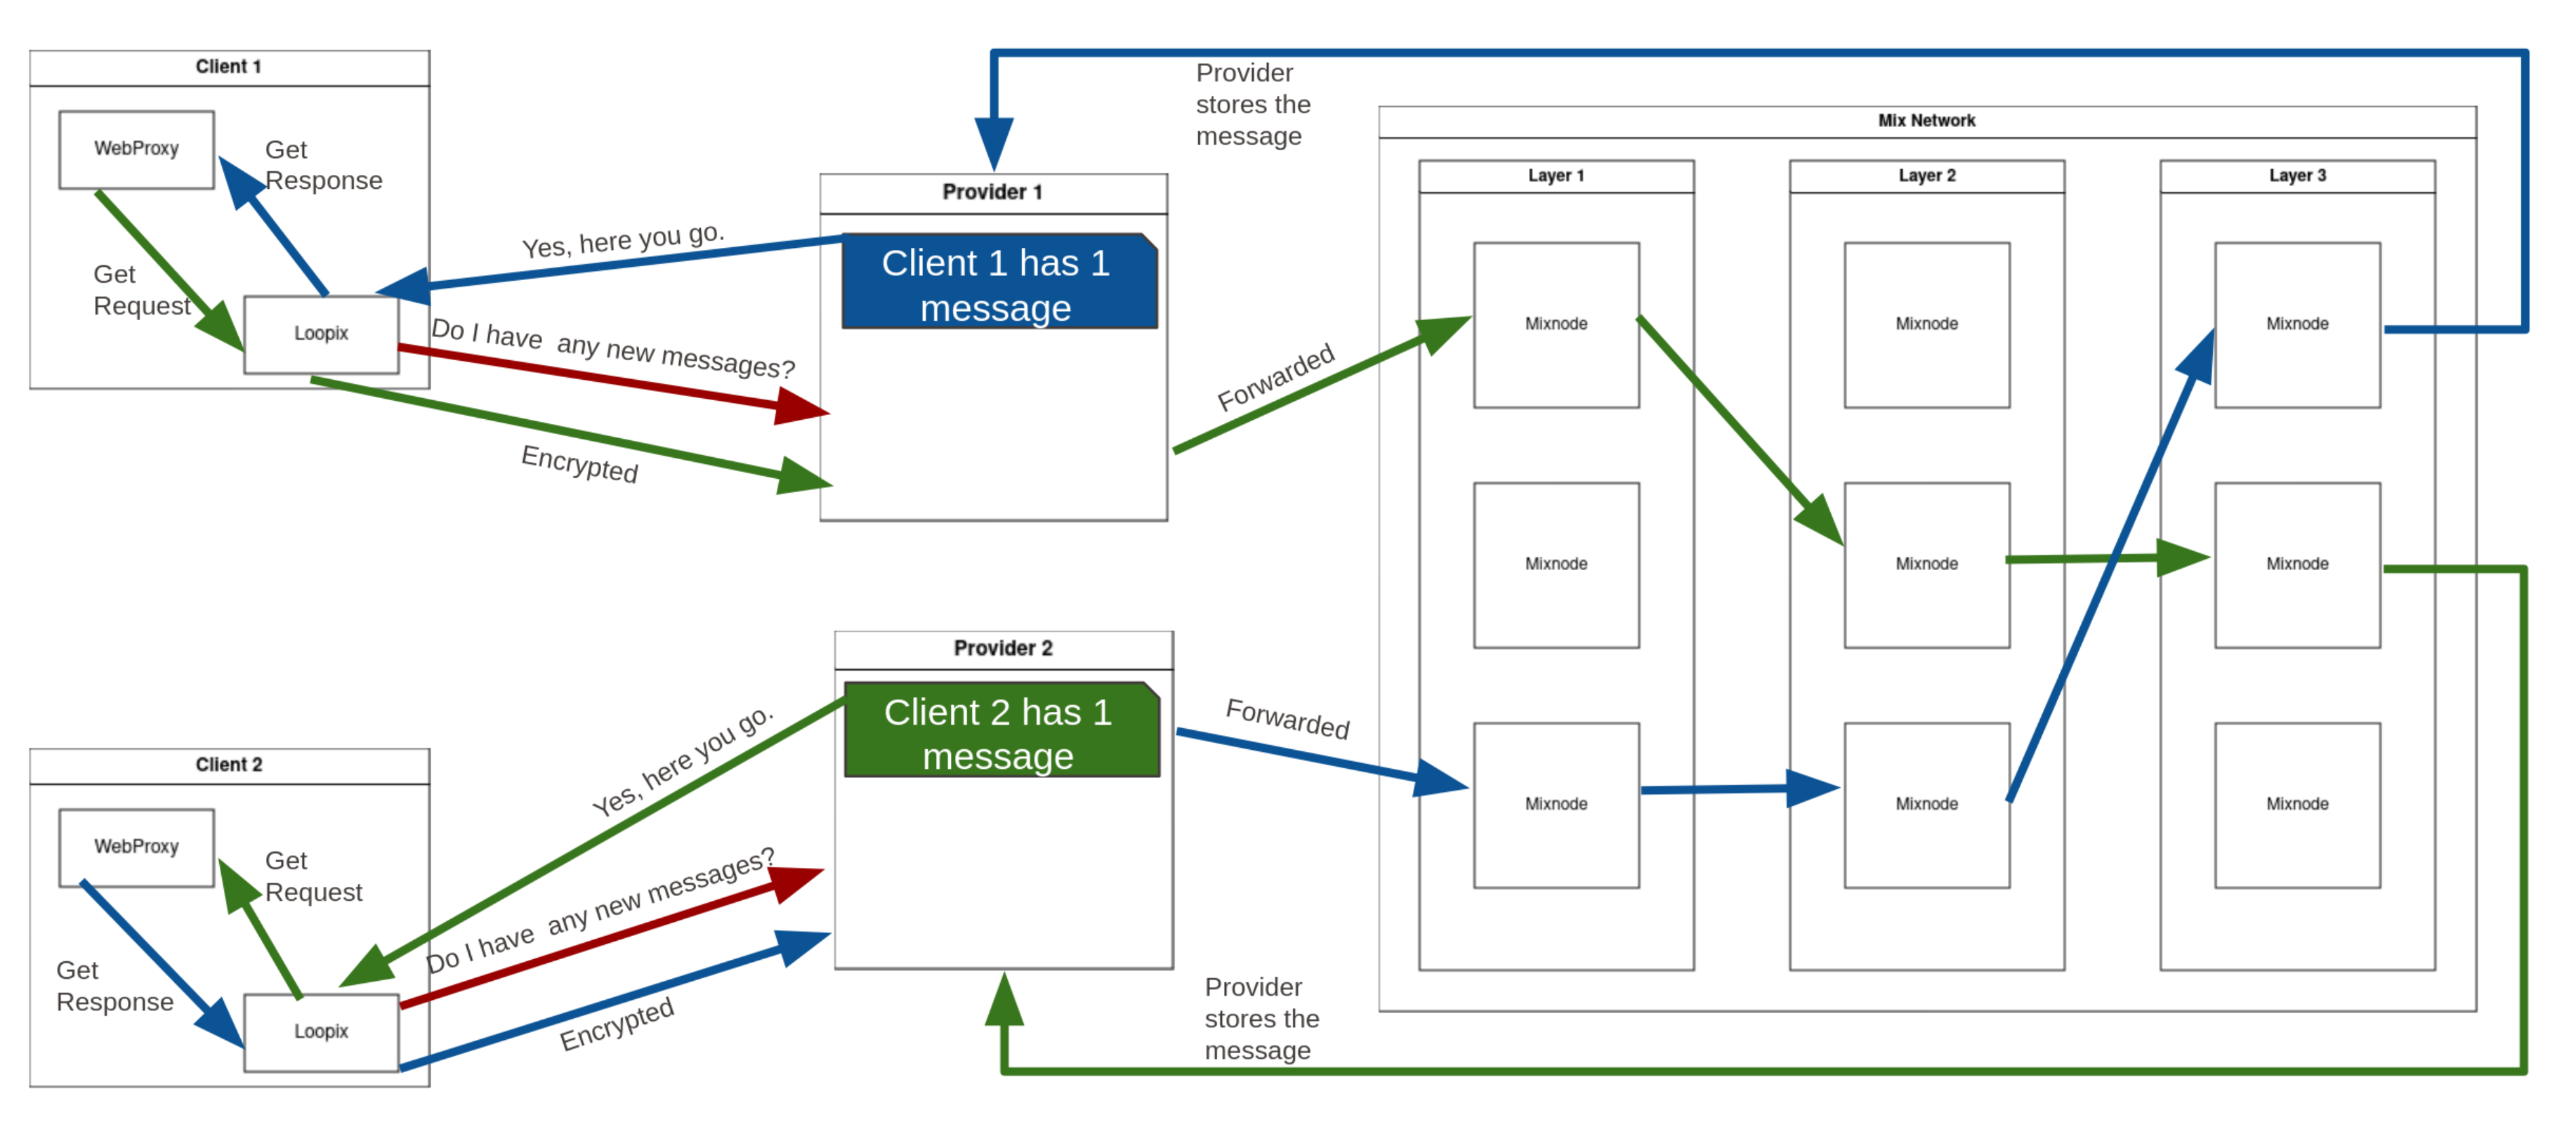
\includegraphics[width=1\linewidth]{plots/implementation.png}
    \caption{}
    \label{fig:implementation}
\end{figure}

%-------------------
\subsection{Assumptions}

\textbf{In an ideal setup with good bootstrapping etc, the threat model is the same as loopix, with the following exception: there has to be enough nodes in the system to  have an anonymity set for the accessed web pages, if the loopix module is used for the sole purpose of transmitting web proxy messages, then an observer definitely knows that a proxy node is receiving messages from a sender (get request is observable), which makes the providers kind of useless}

%-------------------
\subsection{Bootstrapping}
\label{sec:design_bootstrapping}
\textbf{\begin{itemize}
    \item signaling server
    \item nodeID in message (can be fixed with single use reply blocks(!))
    \item unique message ID
\end{itemize}}

\section{Potential Approaches to More Reliable Message Delivery}
\label{sec:reliable_message_delivery}
\textbf{Talk about the simple approach, retrying and duplicate messages, erasure coding and mix groups}

\section{Further Adaptation to Fledger}
\textbf{Briefly describe how retry and duplicate mechanisms work}

\section{Future Work}
\textbf{\begin{itemize}
    \item get rid of providers
    \item bootstrapping and node discovery
    \item faster provider message processing
    \item designing for rid of providers all together
    \item raptor codes (erasure coding)
    \item mix regions
\end{itemize}}

%%%%%%%%%%%%%%%%%%%%%%%%
\chapter{Implementation}
\label{sec:implementation}
%%%%%%%%%%%%%%%%%%%%%%%%

% The implementation covers some of the implementation details of your project.
% This is not intended to be a low level description of every line of code that
% you wrote but covers the implementation aspects of the projects.l

% This section is usually 3-5 pages.
\section{Communication between Modules}
\textbf{Talk about messages and how they wrapped between modules}

\section{Performance Improvements}
\textbf{Two big performance improvements: parallel message processing, stop adding each message to storage :)}

\section{Miscellaneous}
\textbf{Talk using rust sphinx for messages and the one line adaptation needed (maybe I need to talk about it in the background)}

\textbf{Talk about one issue with duplicate messages: web proxy cannot avoid reprocessing (duplicate) responses, it doesn't know how many packets it will receive}

%%%%%%%%%%%%%%%%%%%%
\chapter{Evaluation}
%%%%%%%%%%%%%%%%%%%%

% In the evaluation you convince the reader that your design works as intended.
% Describe the evaluation setup, the designed experiments, and how the
% experiments showcase the individual points you want to prove.

% This section is usually 5-10 pages.
This chapter evaluates the Fledger Loopix module, beginning with an analysis in the absence of churn. It examines how the parameters defined in \autoref{sec:loopix_parameters} were selected specifically for the web proxy application. Subsequently, it investigates the performance of web proxy requests under churn, with and without the use of the reliable message delivery mechanisms detailed in \autoref{sec:reliable_message_delivery}

%-------------------
\section{Experimental Setup}
%-------------------
All simulations were conducted using the Sphere Research Infrastructure \textbf{[cite]}. Each simulation involved 3 clients, 6 mix nodes configured with a path length of 3 (i.e., 2 mix nodes in each layer of the stratified topology), 3 providers, and one signaling server (\autoref{fig:setup}).

The network was emulated with a 50 Mbps link between each node (in a fully connected network) and a network latency of 15 ms. While an ideal setup would involve each node connecting to a single router via individual links, the following sections will demonstrate that network link speed does not present a bottleneck in this context. Additionally, we aim to convince the reader that the Fledger Loopix implementation is scalable to accommodate a significantly larger number of clients.

\begin{figure}[H]
    \centering
    \includegraphics[width=\textwidth]{plots/experimental_setup.png}
    \caption{Experimental Setup}
    \label{fig:setup}
\end{figure}


Each Fledger node in the simulation runs Ubuntu 20.04 LTS with 4 GB RAM and 4 cores on Sphere Testbed Virtual Machines \textbf{link to documentation}. The signaling server node, exceptionally, has 32 GB of RAM and 32 cores to ensure it does not become a bottleneck.

When the simulation begins, client nodes send web proxy requests for the URL \textit{https://ipinfo.io/}. Each client sends one request at a time, waiting for either a successful response or a timeout before sending the next request. All client nodes perform this process concurrently, with each acting as proxy nodes at the same time.

%-------------------
\section{Fine tuning Loopix Parameters for Web Proxy Requests}
\label{sec:finetune}

\textbf{rename the subsections?}

%-------------------
Having implemented the Fledger Loopix module, it is important to ensure that web proxy requests are fast and do not use a lot of bandwidth even in the presence of cover traffic. This section focuses on fine-tuning our implementation with the Loopix parameters described in \autoref{sec:loopix_parameters} to suit the use case of web browsing via a web proxy.

For each experiment, measurements were collected over a 5-minute simulation period. The nodes were given 15 seconds to initialize before the Fledger Loopix module was started. In these simulations, the web proxy timeout, as mentioned in \autoref{sec:fledger_modules}, was set to 20 seconds. This configuration ensures that each request has sufficient time to complete, and any unsuccessful proxy request indicates dropped packets or similar issues.

%-------------------
\subsection{Latency Components}
Before getting into fine tuning the end-to-end latency, it is important to talk about what contributes to the time a proxy request takes. we conducted 12 simulations with identical parameters to show various components of the end-to-end latency. While the average end-to-end latencies are quite stable, it can be noted that there is a variation of 200-400ms between the different simulations.

In \autoref{fig:control_lambdas}, each stacked bar represents the average end-to-end latency for a single simulation round. The dotted red line denotes the actual average end-to-end latency, which is slightly higher than the combined values of all listed components. This discrepancy arises from additional factors, such as the time taken by the proxy node to retrieve the requested website, the preparation of WebRTC messages, and the time required for nodes to set up connections. These elements lie in the gap between the stacked bars and the dotted red line.


\begin{figure}[htbp]
    \centering
    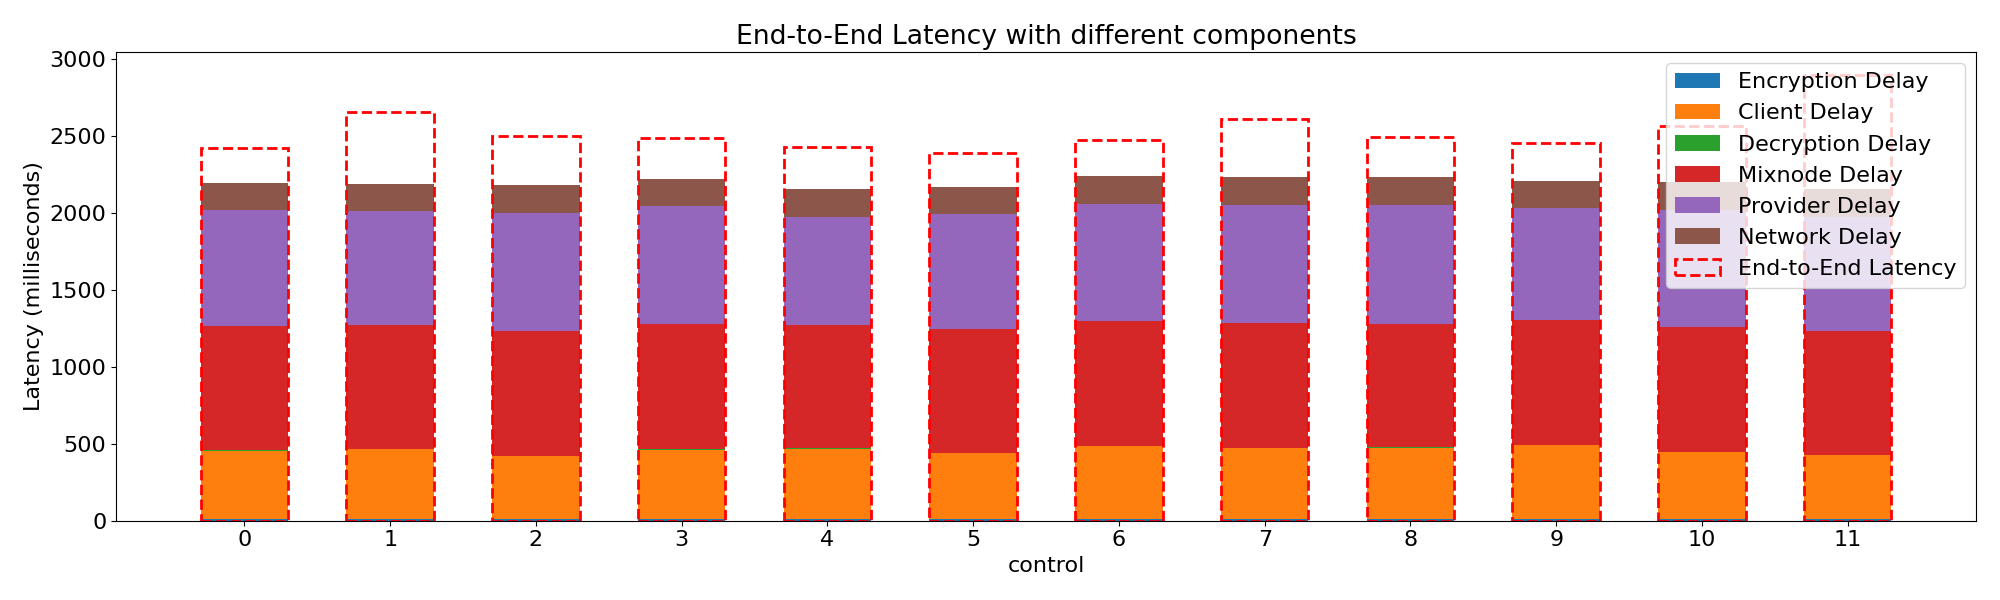
\includegraphics[width=\textwidth]{plots/control_latency_components.png}
    \caption{}
    \label{fig:control_lambdas}
\end{figure}

The figure highlights four major components that significantly contribute to the end-to-end latency, as detailed in the following analysis.

\begin{itemize}
    \item \textbf{Client Delay} \\
    This is the time a message spends waiting in the client’s payload message queue after being created. The Loopix parameter that influences this delay is \(\lambda_P\), which represents the rate (in messages per second) at which the client sends messages from its queue.
    \item \textbf{Mix node Delay} \\
    This refers to the total time a message spends being "mixed," which is the cumulative delay at each layer of the mix network. It approximately corresponds to the formula: (number of layers in the mix network+1) (to account for the provider of the initiating client) multiplied by the the mean delay.  While the graphs display the mean delay observed in the simulations, these delays are drawn from a distribution with a mean \(\mu\). As a result, the average delay at a mix node closely the parameter \(\mu\).
    \item \textbf{Provider Delay} \\
    This is the amount of time a message spends in the storage of the end provider before being sent to the client as part of a pull request response. It is primarily influenced by the \(t_{pull}\) parameter and, to a lesser extent, by \(N_R\) parameter.
    \item \textbf{Network Delay} \\
    The amount of time a packet spends traveling between nodes. In our emulated network, the network delay is set to 15 ms per hop. For a one-way trip, this corresponds to \((l - 1 + 4)*\)15ms, accounting for the following hops: from the sender to the provider, from the provider to the mix network, through the mix network, to the destination provider, and finally to the destination.
\end{itemize}

\autoref{fig:control_lambdas} shows the averages of these values over the course of the simulation in both directions. The legend of the graph also includes the decryption delay and encryption delay, representing the total time spent decrypting Sphinx packets and encrypting payload messages, respectively. However, as these components contribute only minimally to the overall end-to-end latency, they are not prominently visible on the stacked bars.

To highlight one limitation of these measurements, for mix node and decryption delays, the reported values are averages across all messages, including both payload and cover traffic. This is because mix nodes cannot distinguish between payload messages and cover messages.

%-------------------
\subsection{Mean number of messages in the mix}
An important security parameter, described in \autoref{sec:loopix_parameters}, is the mean number of messages in a mix node at a given time. Although the Loopix paper recommends \(\frac{\lambda}{\mu} = 2\) to be at least 2, their experiments are based on providers running on AWS \texttt{m4.16xlarge} instances with 256 GB RAM and mix nodes running on \texttt{m4.4xlarge} with 64 GB RAM. As Fledger is designed as a lightweight program, where a user that wants to participate in the Fledger Loopix network should not need to have a high end machine, we first look into whether or not this recommendation is feasible within our experimental setup.

Since the limiting factor for our nodes with 4 CPU cores would be processing many incoming messages at the same time, in this section we keep \(\mu\) stable and change the number of incoming messages to a mix node per second by adjusting the cover traffic. \(\lambda_L\) and \(\lambda_D\) are set to the same values and adjusted to change the number of incoming messages, while \(\lambda_P\) and \(\lambda_mu\) values are not changed to keep the latency stable.

In the following section \(\mu\) is to 100 ms, which corresponds to a \(\frac{1}{\mu} = \frac{1}{10}\) as a mean delay of 100 ms corresponds to an average of 10 messages leaving the mix node per second. According to the Loopix paper the target value incoming messages per second is 20, where\(\frac{\lambda}{\mu} = \frac{20}{10} = 2\).

\begin{figure}[H]
    \centering
    \begin{subfigure}{\textwidth}
        \centering
        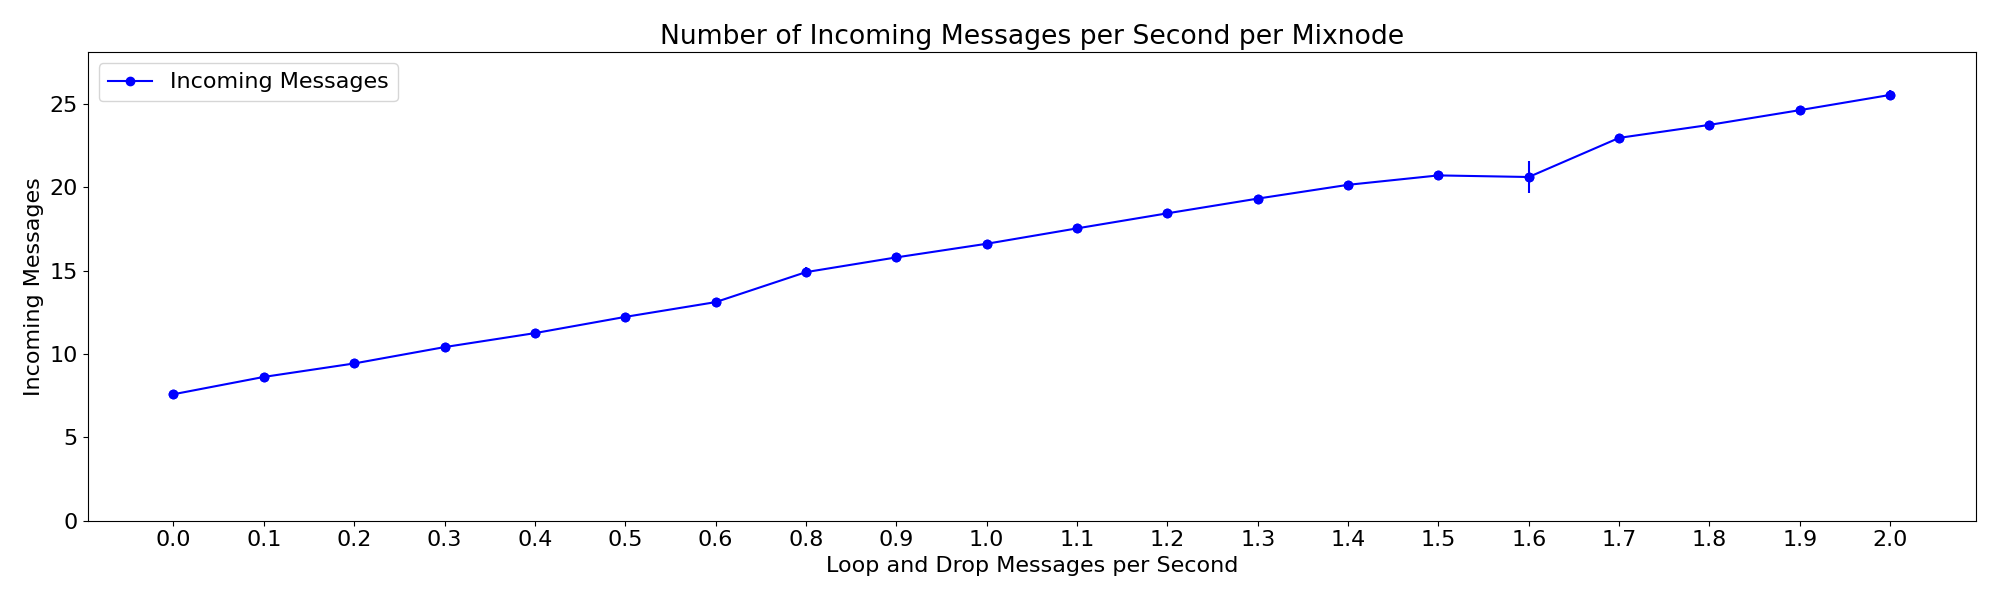
\includegraphics[width=\textwidth]{plots/mu_incoming_messages.png}
        \caption{}
        \label{fig:mu_incoming}
    \end{subfigure}
    \hfill
    \centering
    \begin{subfigure}{\textwidth}
        \centering
        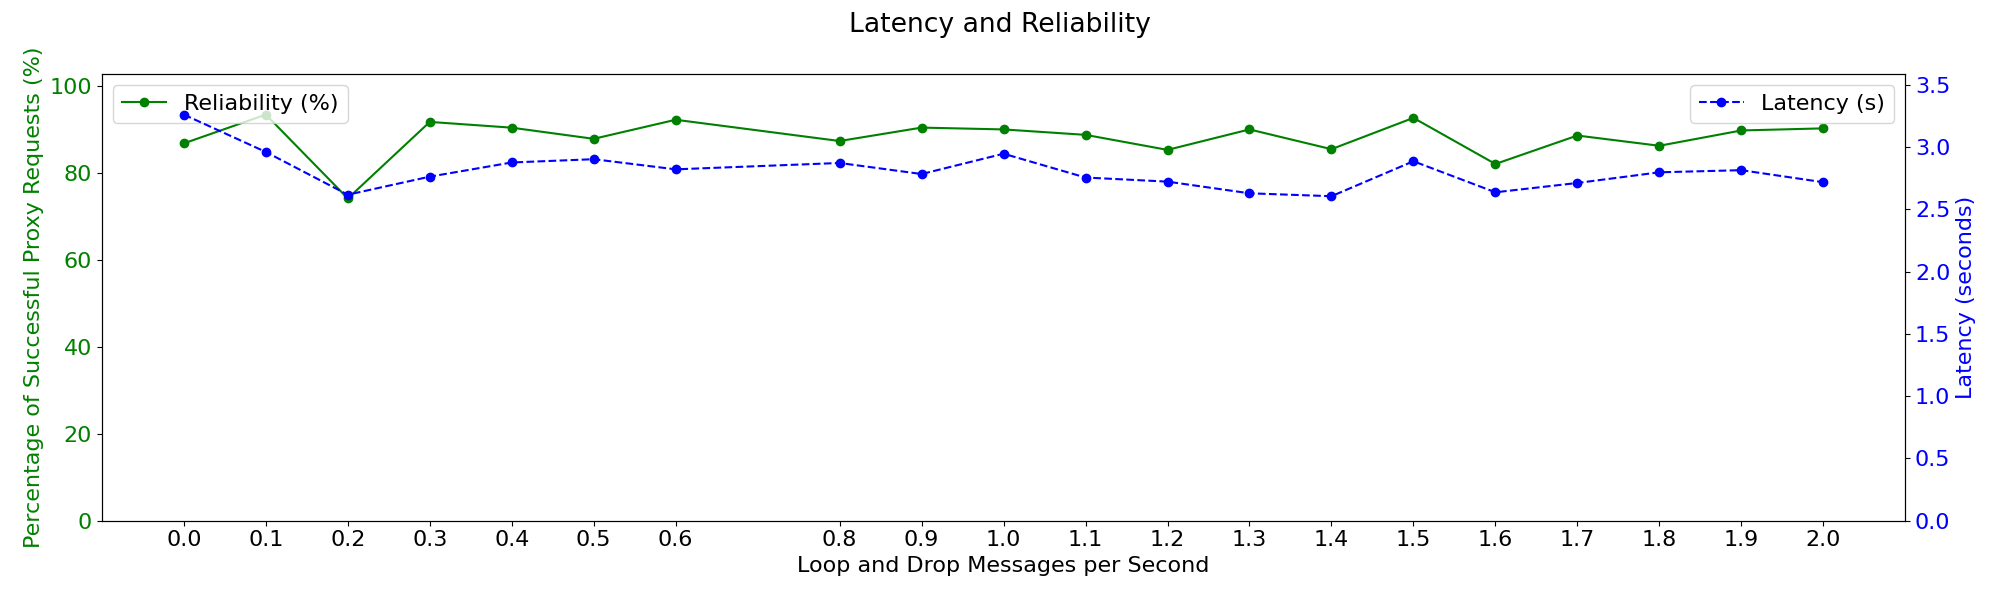
\includegraphics[width=\textwidth]{plots/mu_reliability_latency.png}
        \caption{}
        \label{fig:mu_reliability_latency}
    \end{subfigure}
\end{figure}

\autoref{fig:mu_incoming}, shows that it is possible possible to adjust incoming message by only changing the cover traffic.

In \autoref{fig:mu_reliability_latency} it is possible to see that adjusting the incoming message rate does not affect the percentage of successful proxy requests or the end-to-end latency of the requests.

\textbf{I will run this with more values up a point where the latency and reliability deteriorates, and say that we can use up to X value}

%-------------------
\subsection{Payload Message Rate and Mean Delay}
In the use case of Fledger Loopix with a web proxy, the most critical limitation is the end-to-end latency, as users should be able to browse the internet without experiencing significant delays. This section aims to identify values for \(\mu\) and \(\lambda_P\) that minimize end-to-end latency while maintaining reasonable bandwidth usage.

\subsubsection{Payload Message Rate}
One of the four major components of end-to-end latency is client delay. To reduce this delay, \(\lambda_P\) must be increased. However, to keep the \(\frac{\lambda}{\mu}\) ratio stable, an increase in the payload message rate requires a corresponding decrease in the rates of cover traffic (\(\lambda_L\) and \(\lambda_D\)). The following simulations adjust payload message and cover traffic rates keeping all other parameters the same.

In \autoref{fig:lambdas_latency}, it is possible to see that as payload rate increases, the client delay decreases, which in turn causes the end-to-end latency to decrease, however after a payload rate of 6 messages per second the returns are diminishing. We believe this stems from the fact that creation of these packets puts a a load on the client and the provider. This is supported by \autoref{fig:lambdas_realibility} where as the payload increases the success rate of a web proxy request decreases possibly due to dropped or delayed packets.

\textbf{I should rerun part of this, the cover traffic values towards the end are a bit more than they should be (hence the bandwidth increase)}
In \autoref{fig:lambdas_bandwidth}, we see that increasing the payload rate increases the bandwidth marginally, this is because the incoming message rate also increases \autoref{fig:lambdas_messages}, which indicates that lower cover traffics should have been used in these scenarios.

\textbf{TODO: figure placements}

\begin{figure}[htbp]
    \centering
    \begin{subfigure}{\textwidth}
        \centering
        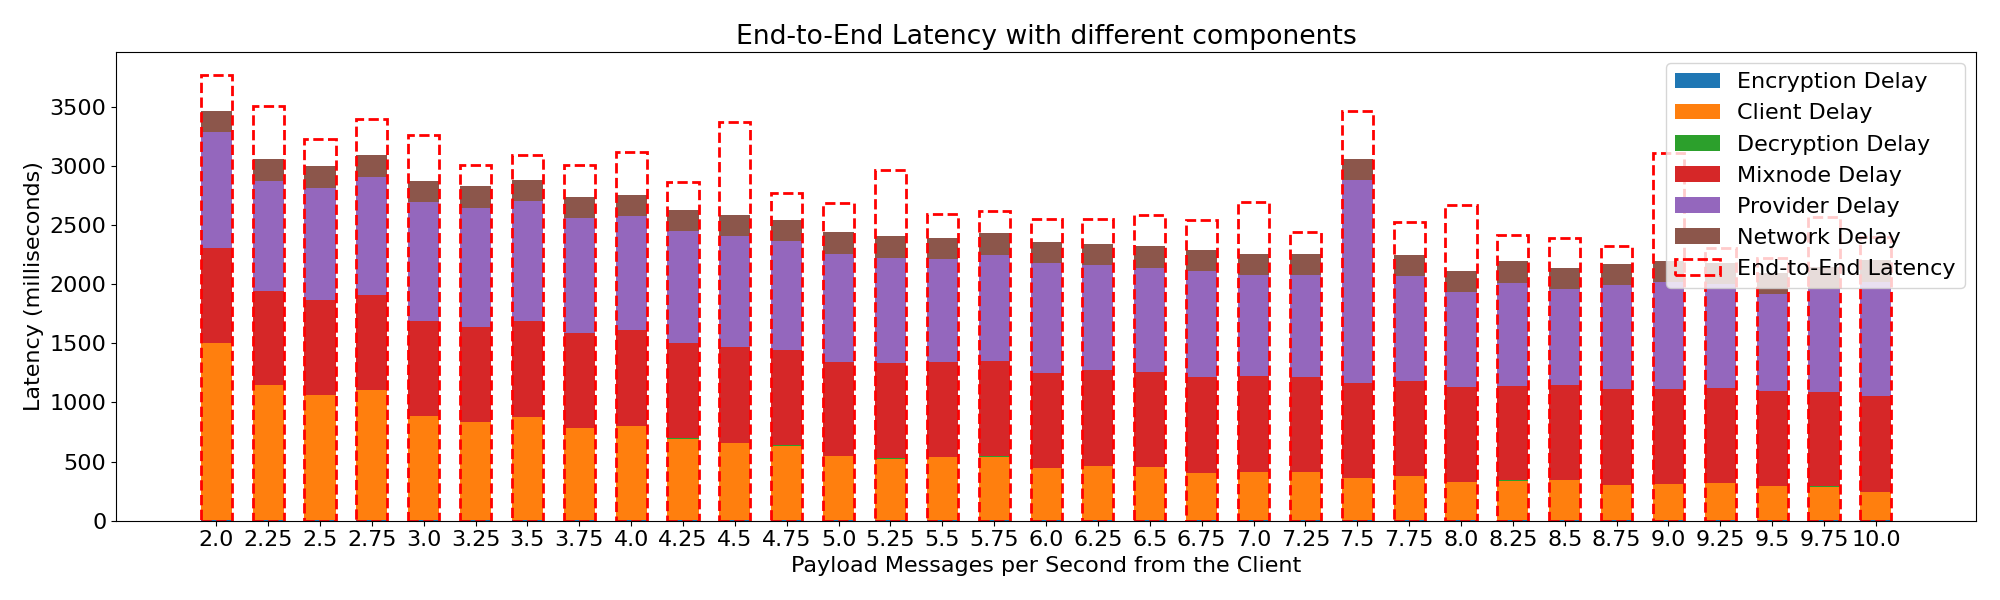
\includegraphics[width=\textwidth]{plots/lambdas_latency_components.png}
        \caption{}
        \label{fig:lambdas_latency}
    \end{subfigure}
    \hfill
    \centering
    \begin{subfigure}{\textwidth}
        \centering
        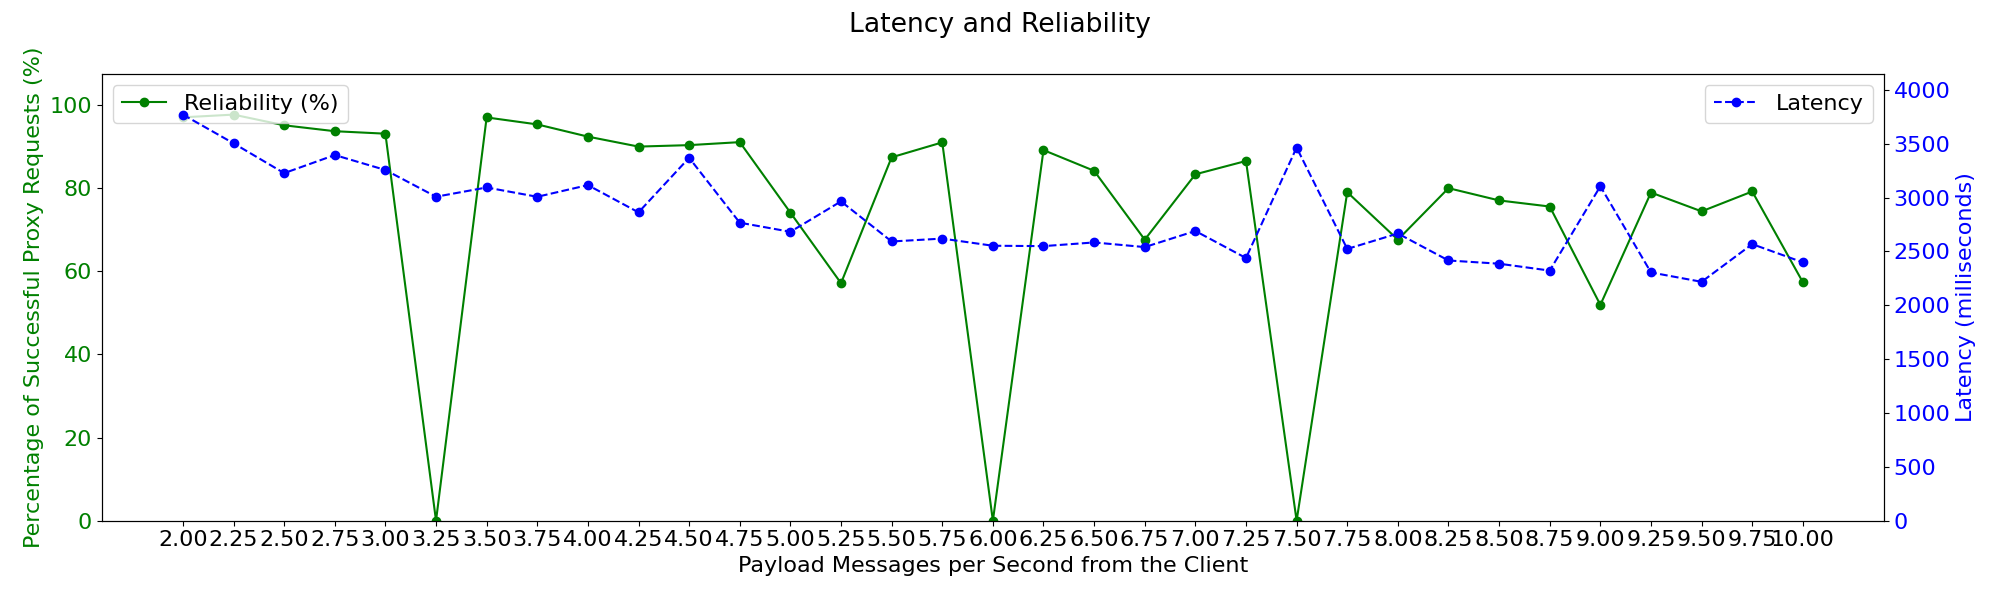
\includegraphics[width=\textwidth]{plots/lambdas_reliability_latency.png}
        \caption{}
        \label{fig:lambdas_realibility}
    \end{subfigure}
    \hfill
    \begin{subfigure}{\textwidth}
        \centering
        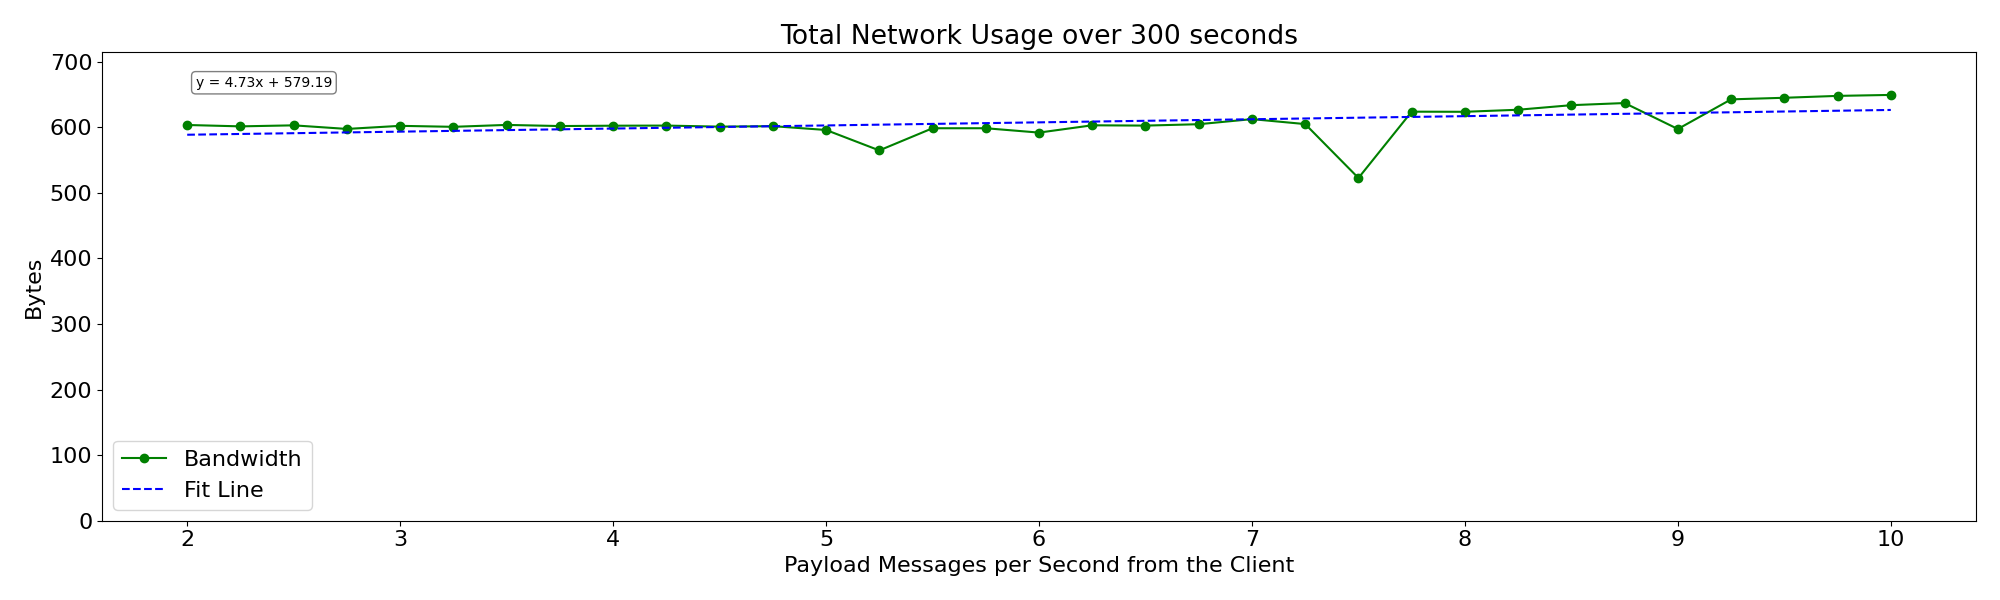
\includegraphics[width=\textwidth]{plots/lambdas_bandwidth.png}
        \caption{}
        \label{fig:lambdas_bandwidth}
    \end{subfigure}
    \hfill
    \begin{subfigure}{\textwidth}
        \centering
        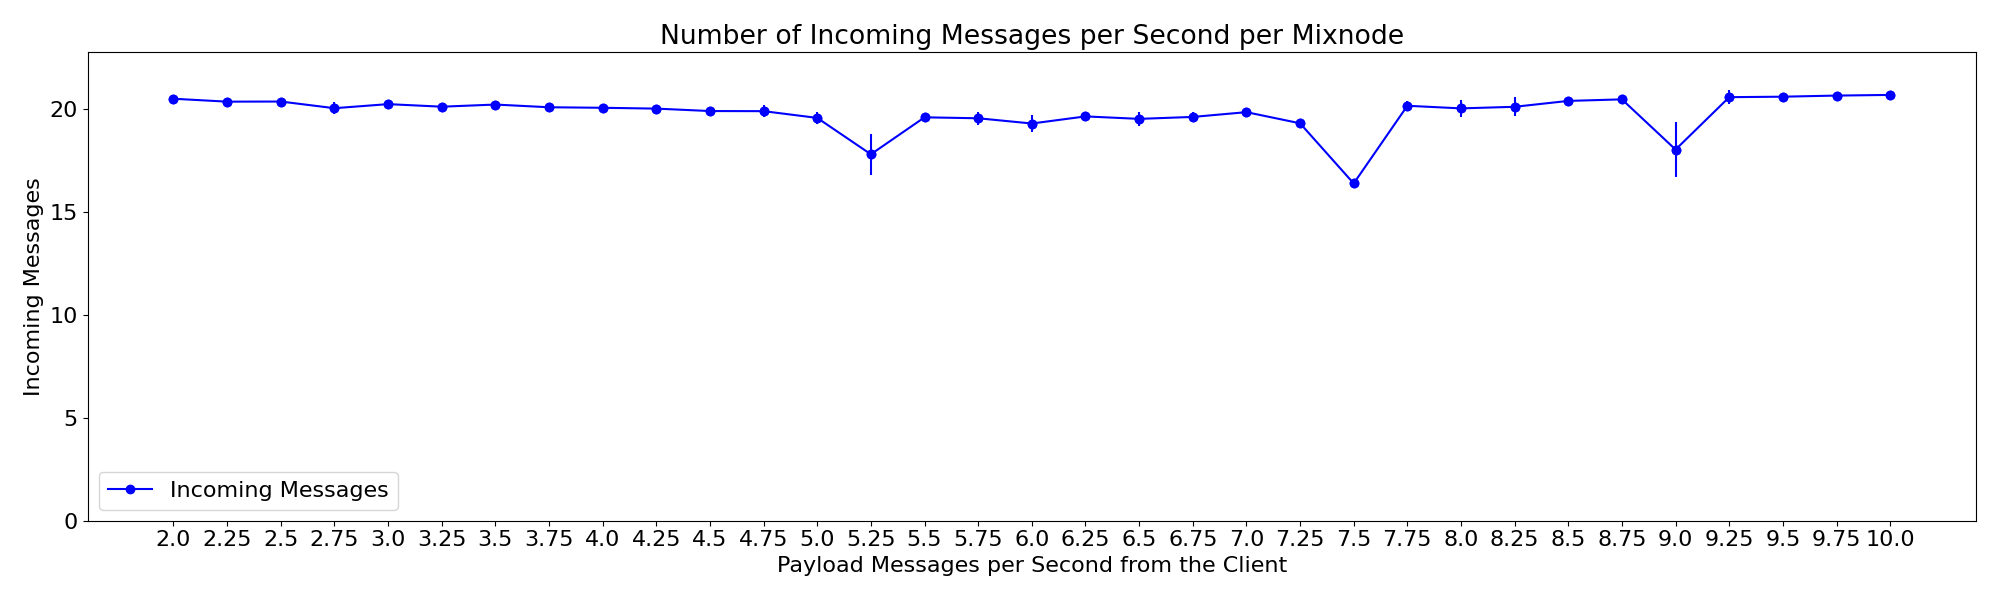
\includegraphics[width=\textwidth]{plots/lambdas_incoming_messages.png}
        \caption{}
        \label{fig:lambdas_messages}
    \end{subfigure}
    \caption{Data visualization for different payload message rates}
\end{figure}


\subsubsection{Mean Delay}
\textbf{Doing the same thing as payload rate with mean delay}
% Next we change mean delay values to see how they change the latency bandwidth etc. Unlike, increasing the payload rate, decreasing the mean delay surprisingly increases reliability. We believe this is due to the worker pool mentioned in \textbf{autoref}, for each forwarded packet a thread is spawned, and this thread is part of the worker pool, therefore less time for the delay means less time for the worker to be released.

% \begin{figure}[htbp]
%     \centering
%     \begin{subfigure}{\textwidth}
%         \centering
%         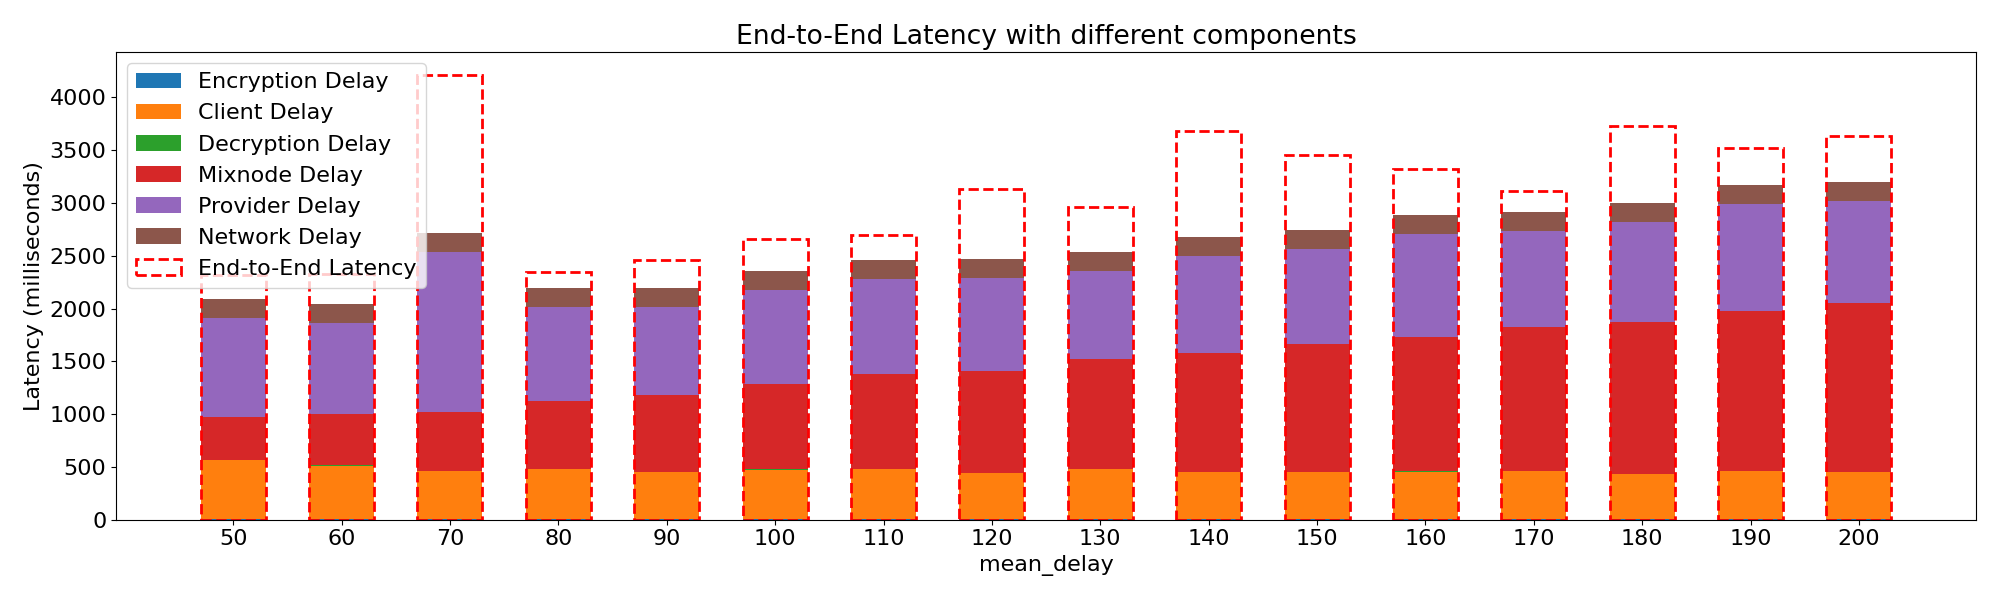
\includegraphics[width=\textwidth]{plots/delays_latency_components.png}
%         \caption{}
%         \label{fig:lambdas_latency}
%     \end{subfigure}
%     \hfill
%     \centering
%     \begin{subfigure}{\textwidth}
%         \centering
%         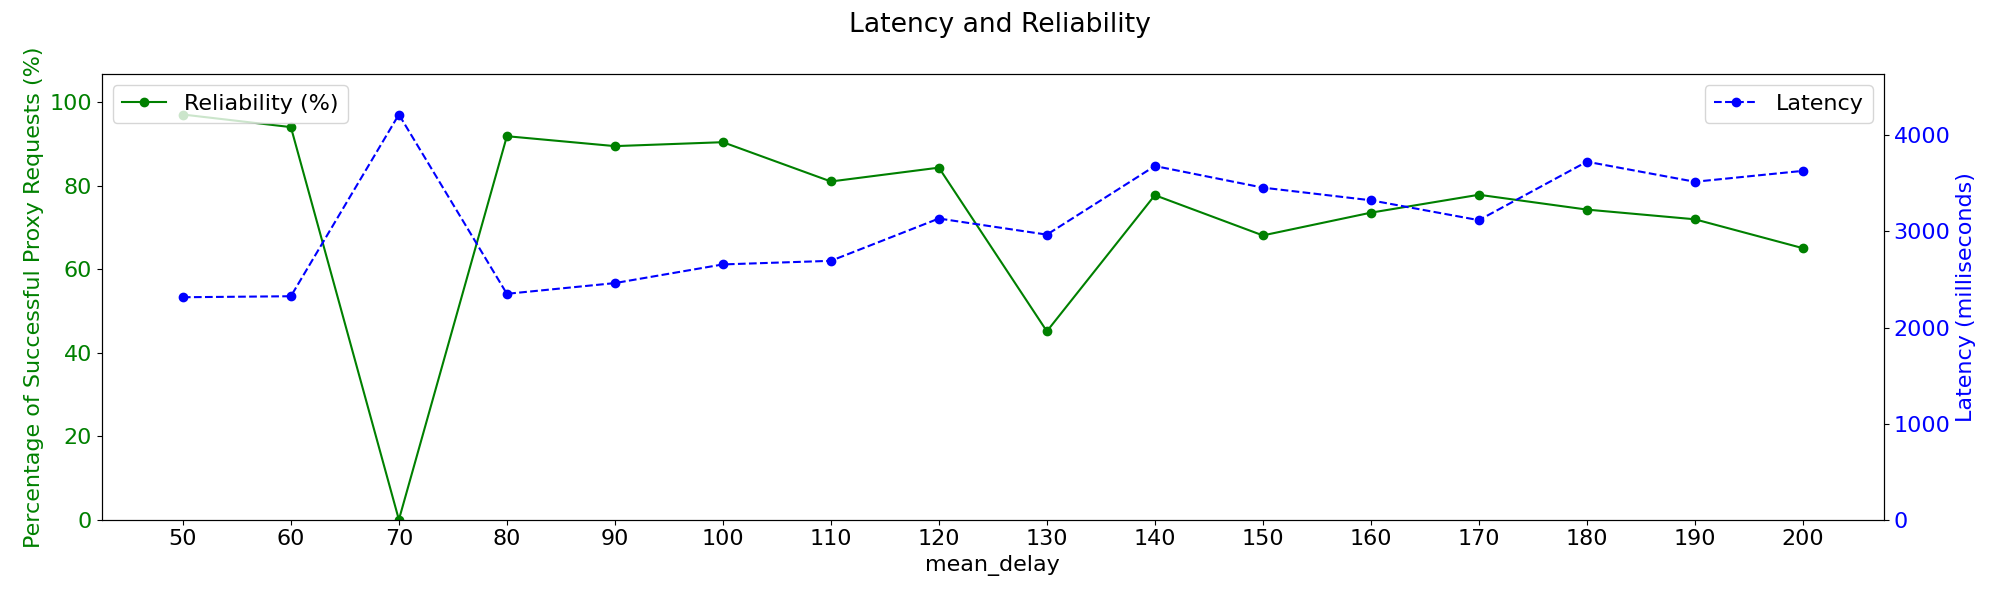
\includegraphics[width=\textwidth]{plots/delays_reliability_latency.png}
%         \caption{}
%         \label{fig:lambdas_realibility}
%     \end{subfigure}
%     \hfill
%     \begin{subfigure}{\textwidth}
%         \centering
%         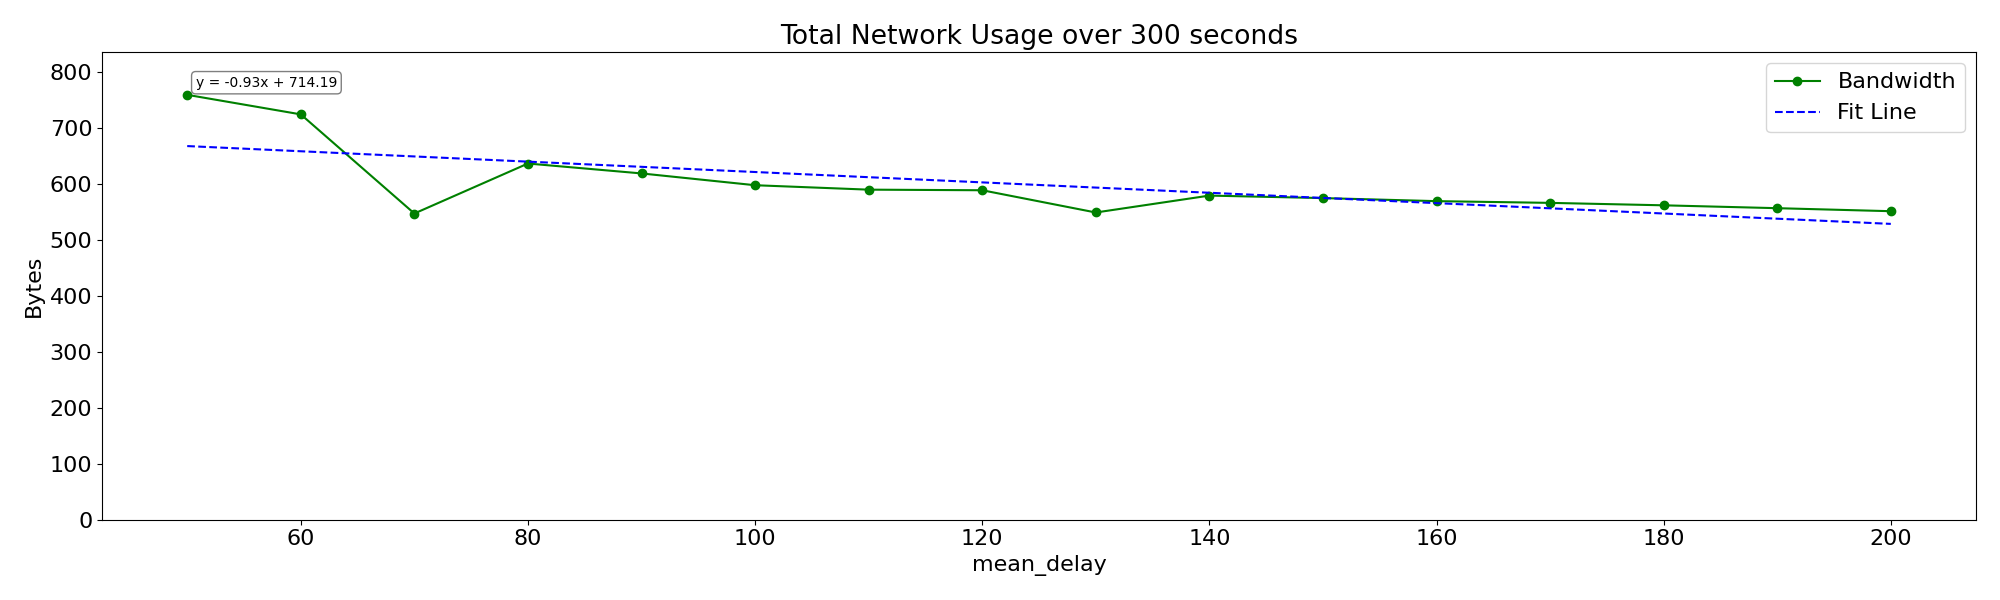
\includegraphics[width=\textwidth]{plots/delays_bandwidth.png}
%         \caption{}
%         \label{fig:lambdas_bandwidth}
%     \end{subfigure}
%     \hfill
%     \begin{subfigure}{\textwidth}
%         \centering
%         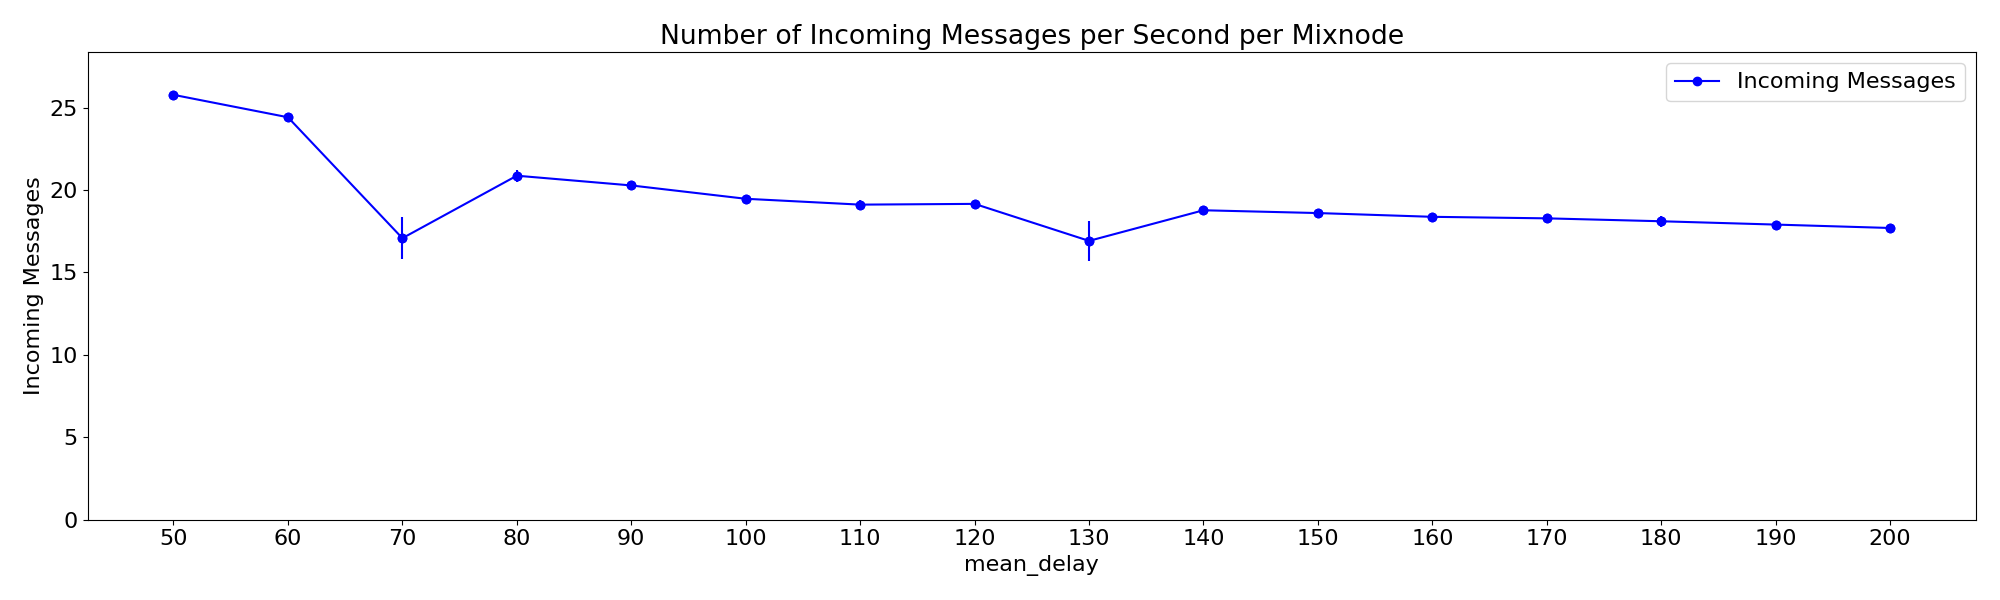
\includegraphics[width=\textwidth]{plots/delays_incoming_messages.png}
%         \caption{}
%         \label{fig:lambdas_messages}
%     \end{subfigure}
%     \caption{Data Visualization for different mean delays}
% \end{figure}

% Since latency decreases and reliability increases, and bandwidth is not affected \textbf{technically shouldn't affected anyway, but I need to rerun a few with less chaff traffic}, we choose 60 as the mean delay going forward. \textbf{link to figures}

%-------------------
\subsection{Choosing Max Retrieve and Time pull}

\textbf{The final big component that contributes to end-to-end latency is provider delay. This delay is related two parameters: \(N_R\) and \(t_{pull}\). This section shows the results of a grid search to find a compromise between end-to-end latency and bandwidth.}

\textbf{insert the heatmaps and discuss what they show}
% In figure \textbf{autoref} there are two heatmaps, one that shows how \(N_R\) and time pull affects total bandwidth and one that shows how these two variables effects end to end latency.
% \begin{figure}[htbp]
%     \centering
%     \begin{subfigure}{\textwidth}
%         \centering
%         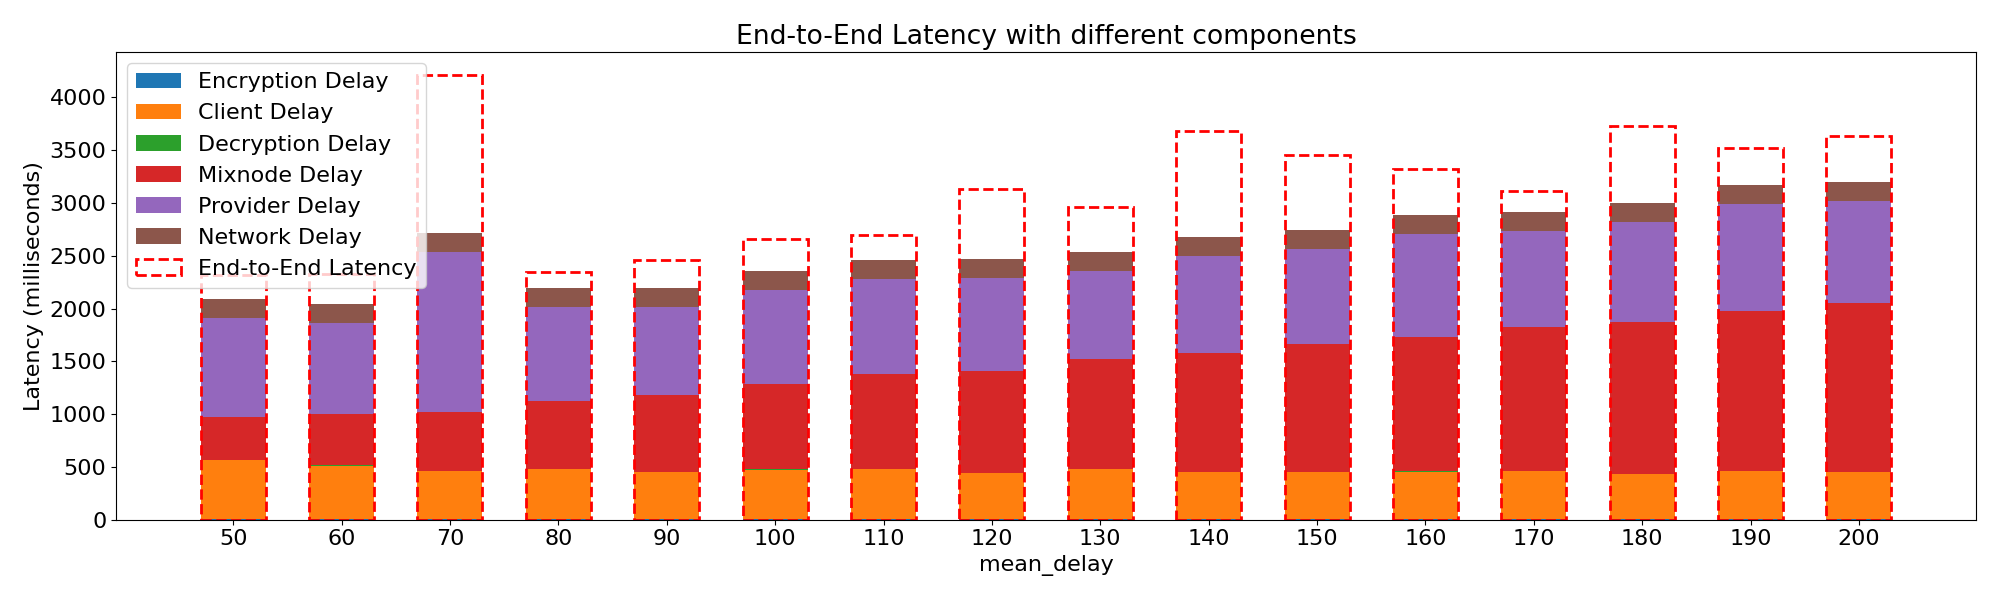
\includegraphics[width=\textwidth]{plots/delays_latency_components.png}
%         \caption{}
%         \label{fig:lambdas_latency}
%     \end{subfigure}
%     \hfill
%     \centering
%     \begin{subfigure}{\textwidth}
%         \centering
%         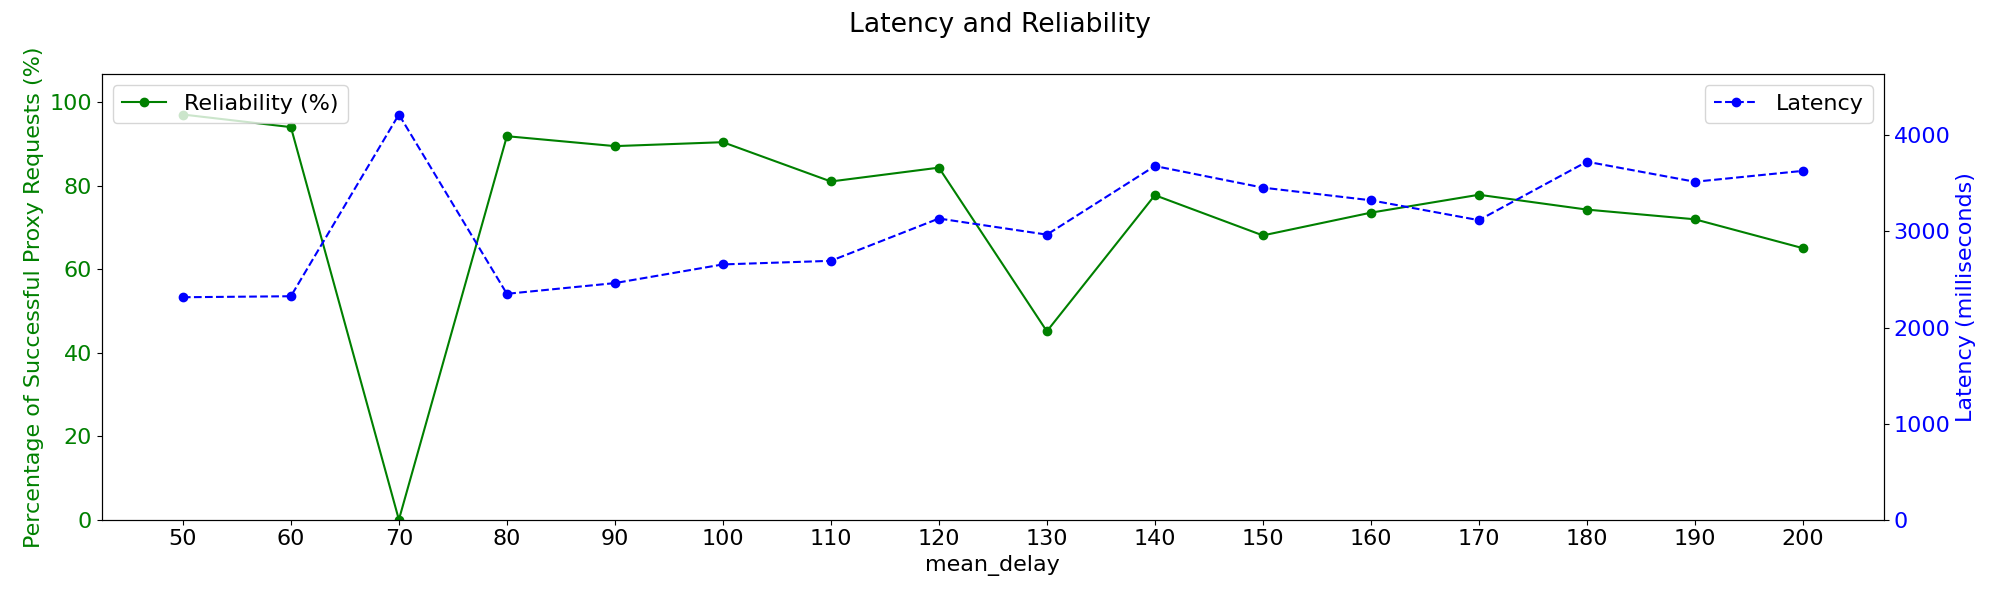
\includegraphics[width=\textwidth]{plots/delays_reliability_latency.png}
%         \caption{}
%         \label{fig:heatmap_bandwidth.png}
%     \end{subfigure}
% \end{figure}


% In \textbf{autoref}, max retreive value over 9 and below 3 increases the latency. We believe below three it is not enough to send the full web page information from the web proxy, and over 9, there is an added overhead for the provider and client to process all the dummy messages which increases latency. As mentioned in \textbf{autoref}, these experiments were run with \textbf{url} proxy requests, and running this experiment with a wider variety of websites would be beneficial. However to accomodate larger websites with multiple body messages from the web proxy, we choose the max retreieve \textbf{X} going forward.

% For time pull it is no surprise that lower time pull decreases latency and increases bandwidth.
% essentially, we believe that as we are tuning our system to browse the internet, we do not need to have a very big max retrieve value but the time pull should be low.


% \textbf{TODO: add plot that shows max retreive average latency over time pulls}

% \textbf{Talk about how we believe removing/replacing the providers would be beneficial and not retract from the anonymity}
% In \textbf{autoref} section, it is mentioned that providers do not serve their main purpose of providing sender receiver online unobservibility. If loopix integration into fledger is only to be used for web proxy module, it might be beneficial to replace providers with simple entry nodes that will not store message but directory send the traffic to the client. \textbf{The client needs to know the network anyway, so they're kinda useless here} Mixnodes in the first and final layers of mix network could be used for this purpose, and would significantly reduce end-to-end latency while not affecting privacy properties. However, if fledger loopix module would be used for other purposes such as private messaging, providers could still provide better privacy than not. We leave this extension/study of fledger loopix module to future work.

%-------------------
\subsection{Scalability}
\textbf{Show that keeping the incoming message rate per mix node is possible through adjusting the cover traffic when new nodes join the network (in different runs)}
% Although we were not able to set up a experiments with larger number of nodes, in this section we try to demonstrate that this integration of Loopix Anonymity System into Fledger is scalable to many more nodes in the network. The same way we changed the cover traffic volume to accomodate the change in payload values and mean delay to keep the \textbf{mean number of messages at a mixnode} the same, we can adjust cover traffic to accomodate changing number of mixnodes and clients.

% \textbf{insert graphs}
% Here we show, path length two, 2 clients, 5 and 10 clients each with the same latency and incoming messages, but adjusted volume of cover traffic. As long as the providers can accomodate the incoming messages from many clients, loopix integraion into fledger is scalable. \textbf{as mentioned in autoref, ideally we would get rid of providers all together.}

%-------------------
\section{Reliability Mechanisms}
%-------------------
\textbf{In section this section, each measurement is taken within a simulation of 1235 seconds  (\(\approx 20\) minutes). The nodes are again allowed get started for 15 seconds, after which Fledger Loopix module is started. After about 5 minutes of normal operations, one of the mix nodes at the first layer is stopped, after another 5 minutes one of the mix nodes at the second layer stopped, and finally after another 5 minutes, one of the mix nodes at the final layer of the mix network is stopped. The simulation continues to run for another 5 minutes with only one node at each layer, while the clients are unaware that the mix nodes are not operational.}

\textbf{Here the web proxy timeout is set to 6 seconds, approximately 2-3 times the average latency with this configuration. The timeout is set to this value to be able to study the effectiveness of the mechanisms in this section.}
%-------------------
\subsection{Retrying}

%-------------------
\subsection{Duplicate Messages}

%-------------------
\subsection{Combination of Retrying and Duplicate Messages}

%%%%%%%%%%%%%%%%%%%%%%
\chapter{Related Work}
%%%%%%%%%%%%%%%%%%%%%%

% The related work section covers closely related work. Here you can highlight
% the related work, how it solved the problem, and why it solved a different
% problem. Do not play down the importance of related work, all of these
% systems have been published and evaluated! Say what is different and how
% you overcome some of the weaknesses of related work by discussing the 
% trade-offs. Stay positive!

% This section is usually 3-5 pages.

\textbf{I will probably skip this because of sections \autoref{sec:mixers} and \autoref{sec:reliable_message_delivery}}

%%%%%%%%%%%%%%%%%%%%
\chapter{Conclusion}
%%%%%%%%%%%%%%%%%%%%

% In the conclusion you repeat the main result and finalize the discussion of
% your project. Mention the core results and why as well as how your system
% advances the status quo.

\cleardoublepage
\phantomsection
\addcontentsline{toc}{chapter}{Bibliography}
\printbibliography

% Appendices are optional
% \appendix
% %%%%%%%%%%%%%%%%%%%%%%%%%%%%%%%%%%%%%%
% \chapter{How to make a transmogrifier}
% %%%%%%%%%%%%%%%%%%%%%%%%%%%%%%%%%%%%%%
%
% In case you ever need an (optional) appendix.
%
% You need the following items:
% \begin{itemize}
% \item A box
% \item Crayons
% \item A self-aware 5-year old
% \end{itemize}

\end{document}